\chapter{User Manual}
\label{user_manual}
\settocdepth{chapter}

\section{Ikke innlogget}

\subsection{Forside}
\begin{center}
  \makebox[\textwidth]{
  \includegraphics[height=80mm, width=\paperwidth-15mm]
  {appendix/manualPictures/A-home-login-cut.png}
  }
\end{center}
\begin{enumerate}[nosep]
    \item Navigasjons bar, som viser tilgjengelige sider. Den blå steken under en side, viser hvilken side du er på nå.
    \item Denne blir bare synlig, hvis brukeren trykker på knappen ”Logg inn”, som vist under punkt 1.
    \begin{enumerate}
        \item Innlogging hvis brukeren har allerede registrert bruker, uten Facebook
        \item Trykk på denne knappen for a logge inn ved bruk av Facebook konto. Åpner nytt vindu, hvor man skriver inn Facebook brukernavn og passord, hvis man ikke er logget inn på Facebook i samme nettleser. Er man det logges man direkte inn.
        \item Trykk her får å bli navigert til side for å registere ny bruker (se: ny bruker) uten Facebook, slik at man kan benytte seg av 2.3.
    \end{enumerate}
    \item vises de 4 førstkommende aktiviteter som er registrert på Skalvi.no. Aktivitetene er sortert på dato. 
    \begin{enumerate}
        \item Et slikt kort / flis representerer en aktivitet. For mer informasjon om en aktivitet, trykk på ønsket aktivitet og en boks (se: modal\_annonym) med informasjon vil poppe opp i forgrunn av siden.
    \end{enumerate}
    \item Her vises versjon nummer. Versjon 1.0.0 er første utgivelse av Skalvi.no.
    \item Her spesifiseres det hvilken lisens Skalvi.no er utviklet under. Apache2.0 er en åpen kildekode lisens.
    \item Her er alle navnet til alle utviklerne av Skalvi.no og gruppemedlemmene som jobbet med bachelor oppgaven UngIT.

\end{enumerate}

\subsection{Registrer ny bruker}
\begin{center}
  \makebox[\textwidth]{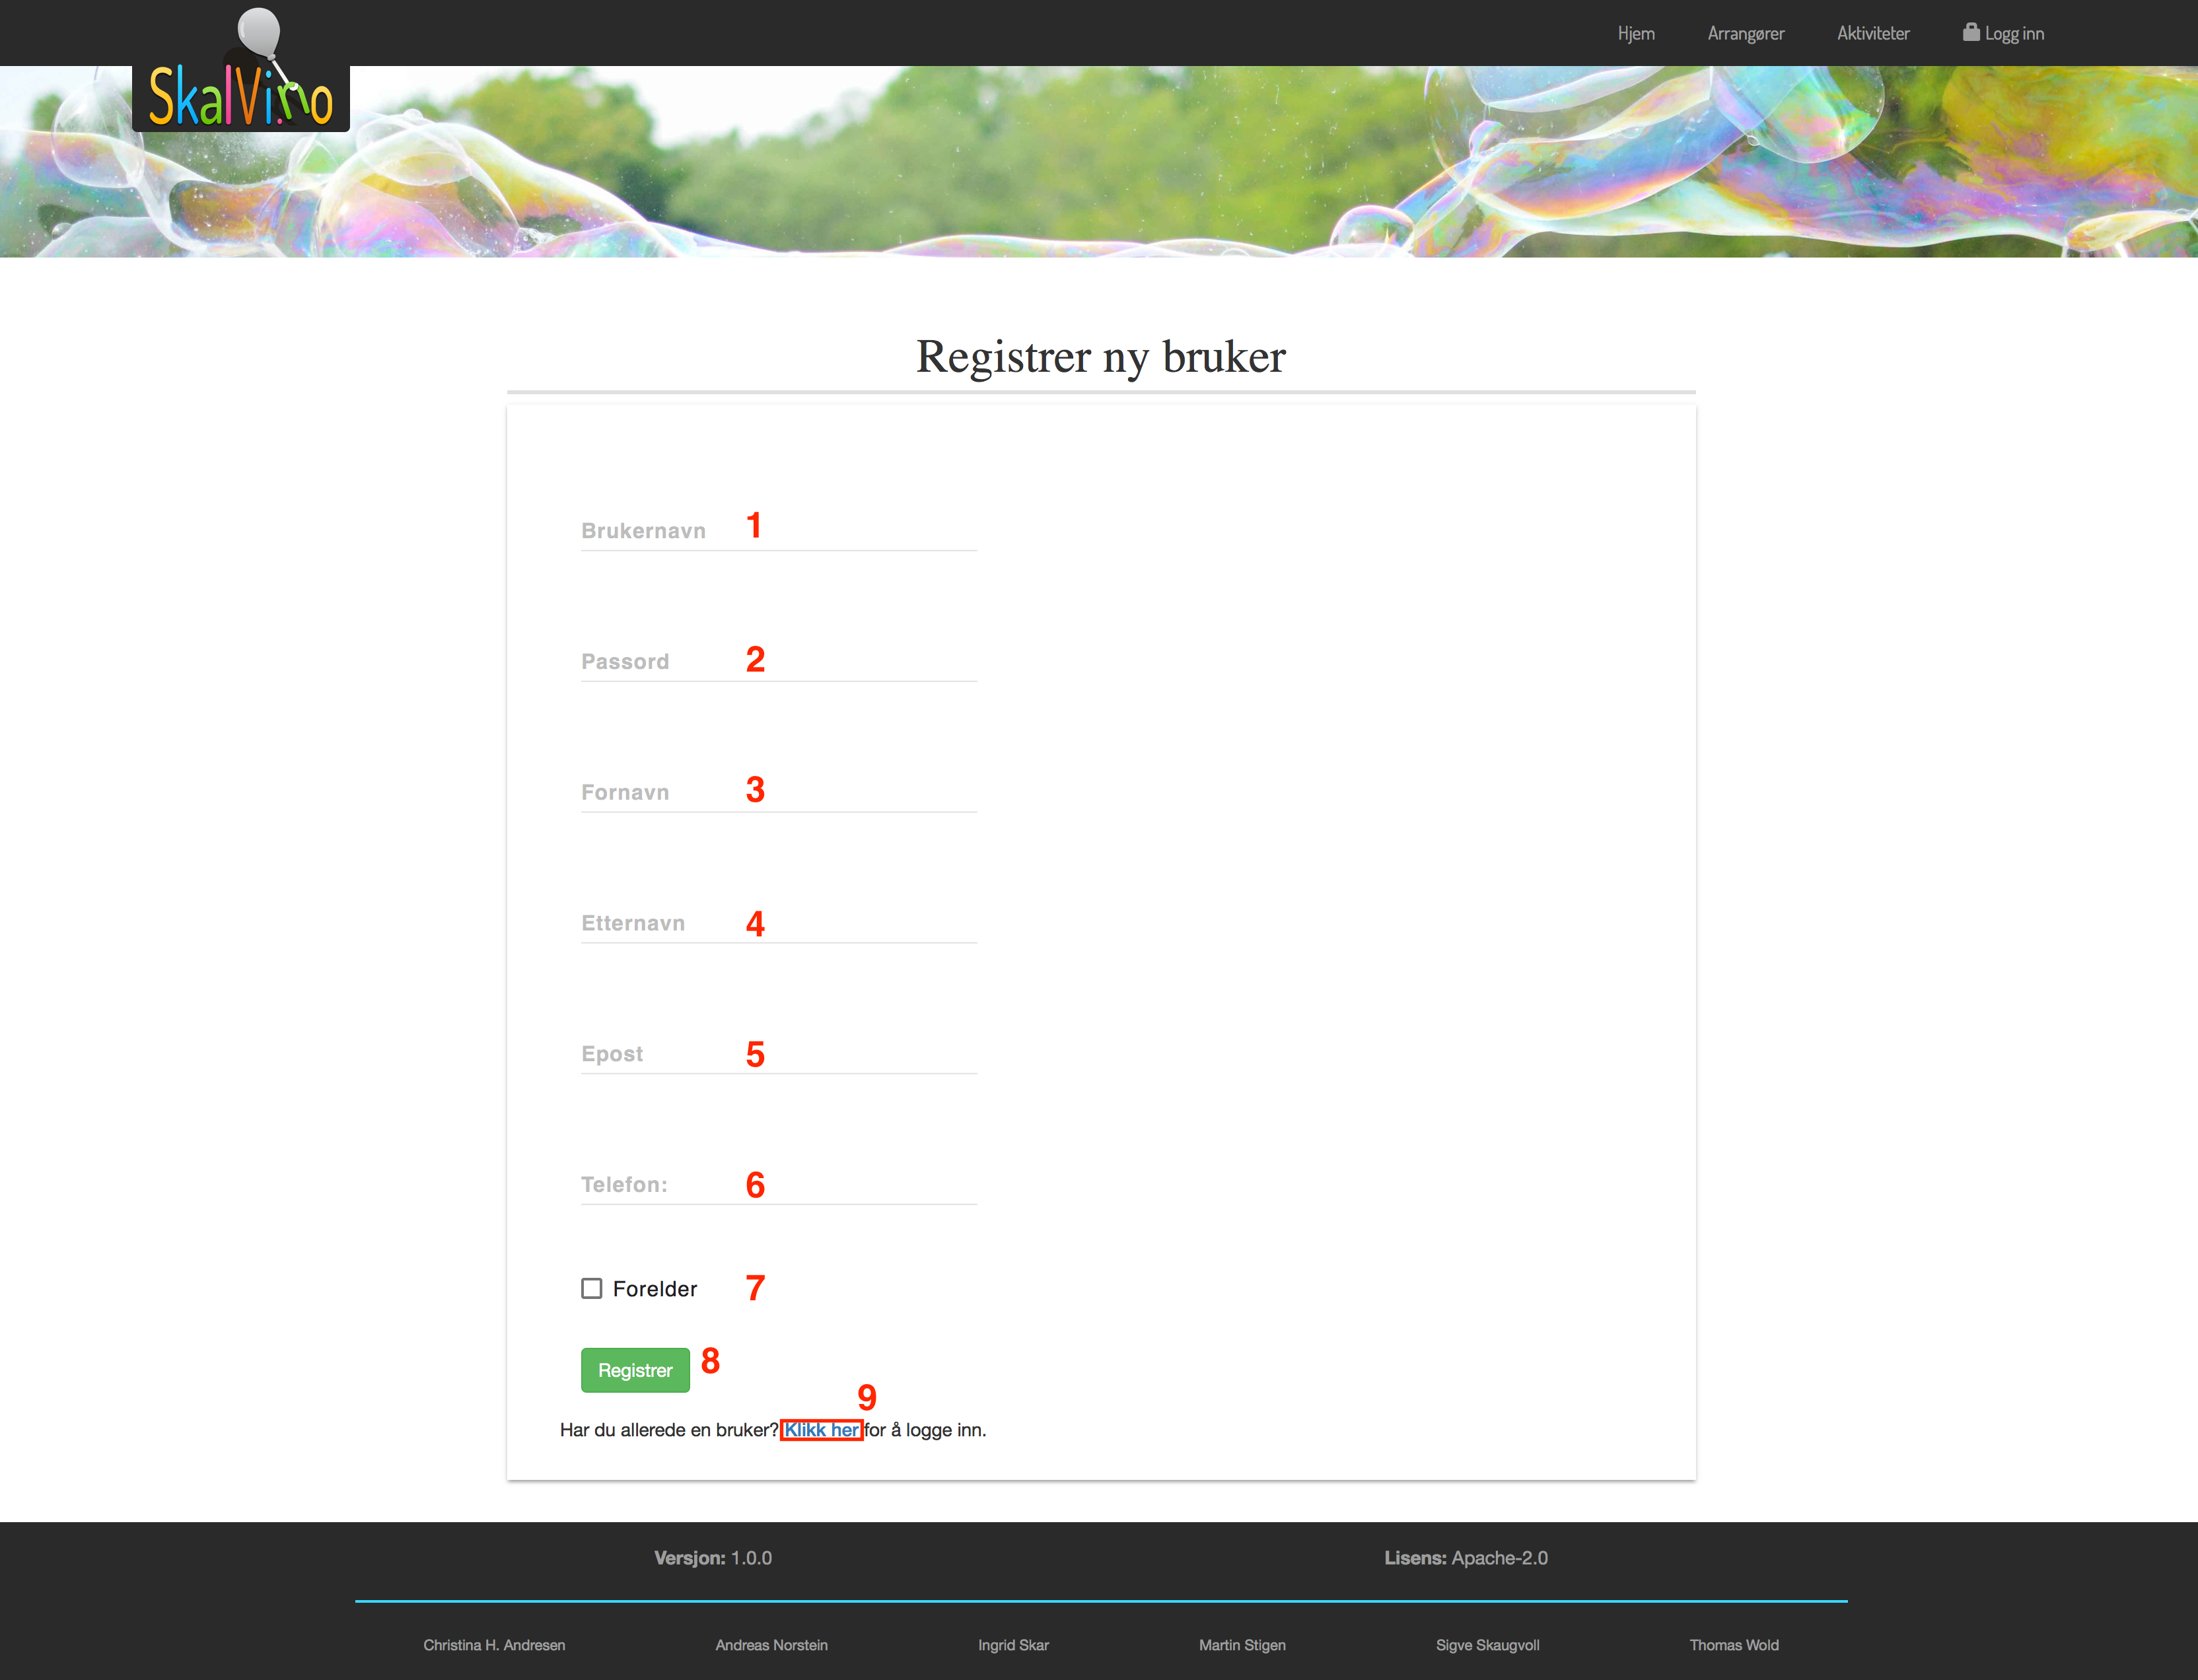
\includegraphics[height=80mm, width=\paperwidth-15mm]{appendix/manualPictures/A-newUser-cut.png}}
\end{center}
\begin{enumerate}[nosep]
    \item Felt for å skrive inn brukernavn til familiebrukeren (hovedprofilen)
    \item Felt for å skrive inn passord til familiebrukeren (hovedprofilen),  vil bli vist som svarte dotter, når skrevet inn, Dette av sikkerhetsgrunner.
    \item Felt for å skrive inn fornavn til hovedprofilen
    \item Felt for å skrive inn etternavnet til hovedprofilen
    \item Felt for å skrive inn Epost til familiebrukeren
    \item Felt for å skrive inn Telefon nummer til familiebrukeren
    \item Velg denne hvis hovedprofilen til familiebrukeren er en forelder.
    \item Trykk her får å registrere familiebrukeren. Hovedprofil blir automatisk opprettet og aktiv bruker.
    \item Trykk her hvis du allerede har registrert en bruker før, det gjelder også hvis du har logget inn med Facebook tidligere.
\end{enumerate}

\subsection{Modal}
\begin{center}
  \makebox[\textwidth]{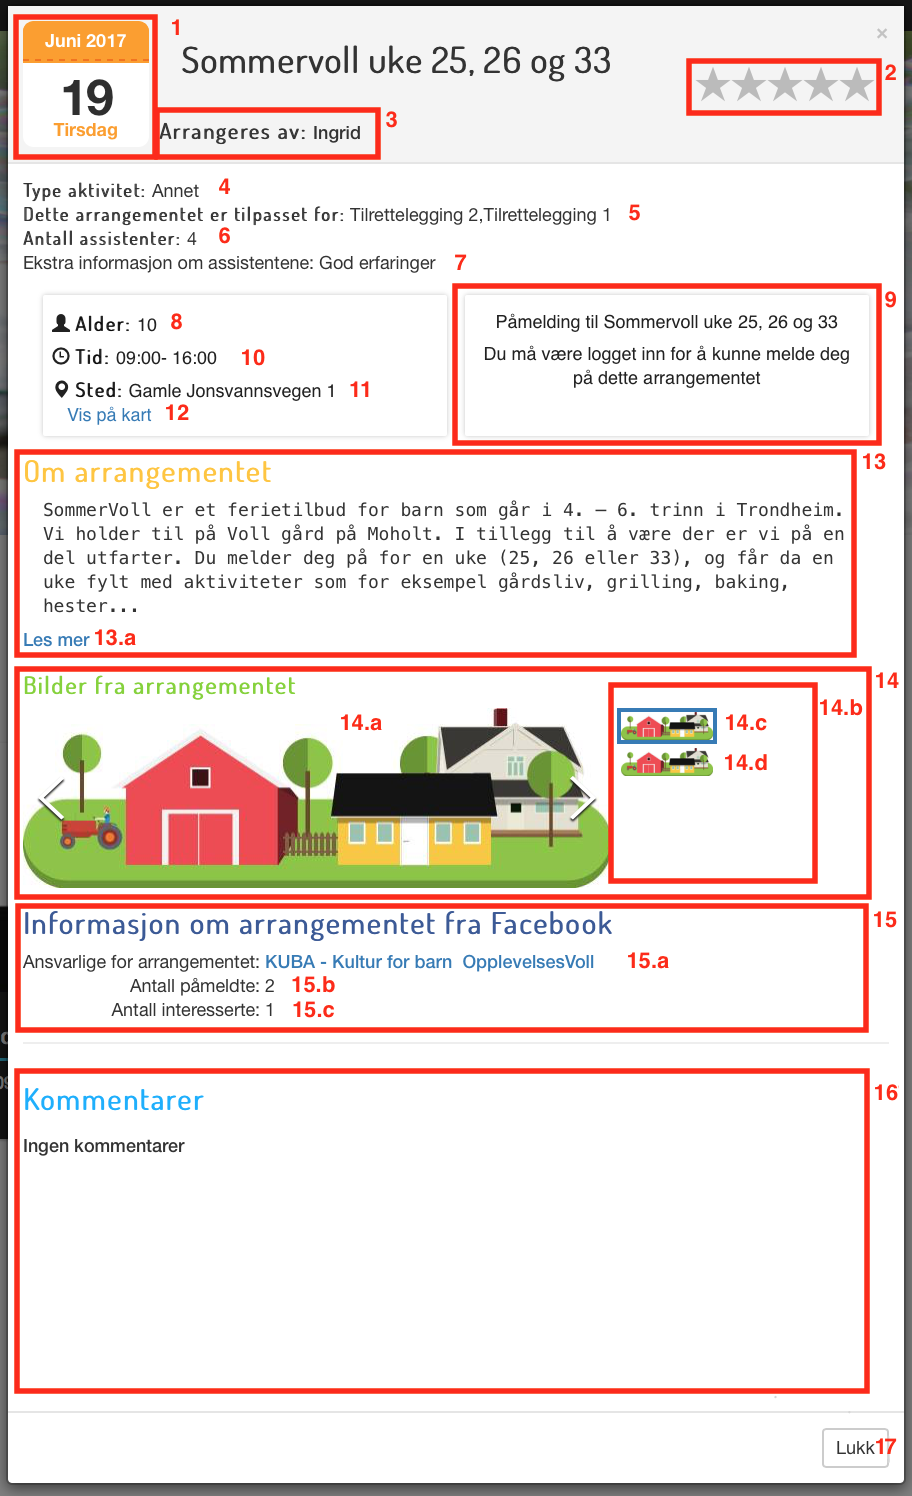
\includegraphics[height=130mm,width=\paperwidth-15mm]{appendix/manualPictures/A-modal-cut.png}}
\end{center}
\begin{enumerate}[nosep]
    \item Dato for aktivitet
    \item Hvis aktiviteten har en rangering, vil stjernene være gul farget og representere rangeringen
    \item Hvem som er ansvarlig for aktiviteten, og dens informasjon på Skalvi.no
    \item Hvilken type aktivitet
    \item Hvem aktivitene er tilrettelagt for, dette skal i videre utvikling bli erstattet med symboler. Og dermed bli mer synlig.
    \item Hvor mange assistenter, dette skal fjernes i vider utvikling på grunnlag av bruker tilbakemeldinger
    \item Ekstra informasjon om assistene i punkt 6. 
    \item Aldergruppe, fra og oppover.
    \item Hvis brukeren logger inn, vil det vises en meld på knapp. Informerer nå brukeren om at de må logge på for å kunne melde seg på.
    \item Tidspunkt aktiviteten startet og slutter
    \item Hvor aktiviteten skal forekomme.
    \item En knapp som vil åpne en ny nettleser fane og vise på Google Maps hvor aktiviteten skal forekomme.
    \item Utdypende informasjon og forklaring om aktiviteten. 
    \begin{enumerate}
        \item For å lese all teksten som er registrert, trykk her. Da vil boksen (punkt 13.) utvide seg og viser mer utfyllende informasjon
    \end{enumerate}
    \item Her vil bilder fra og om aktiviteten vises.
    \begin{enumerate}
        \item Her vil bilde som er markert med blå (14.c) i boks 14.b,  vises. 
        \item Her vil alle bilder som er lastet opp vises, brukeren kan velge å trykke på et bilde for at det skal vises som 14.a
        \item Blå markering, viser hvilket bilde som er aktivt og vises i 14.a
        \item Bilde som er tilgjengelig, men vises ikke i 14.a
    \end{enumerate}
    \item Hvis aktiviteten er hentet fra Facebook, står det her, 
    \begin{enumerate}
        \item hvem som har laget og arrangerer aktiviteten på Facebook
        \item Hvor mange personer som har trykket ”Skal” på Facebook arrangementet
        \item Hvor mange personer som har trykket ”Interessert” på Facebook arrangementet.
    \end{enumerate}
    \item Her vil alle kommentarer som er skrevet på Skalvi.no om denne aktiviteten vises. 
    \item Knapp for å lukke modalen.
\end{enumerate}

\subsection{Arrangører}
\begin{center}
  \makebox[\textwidth]{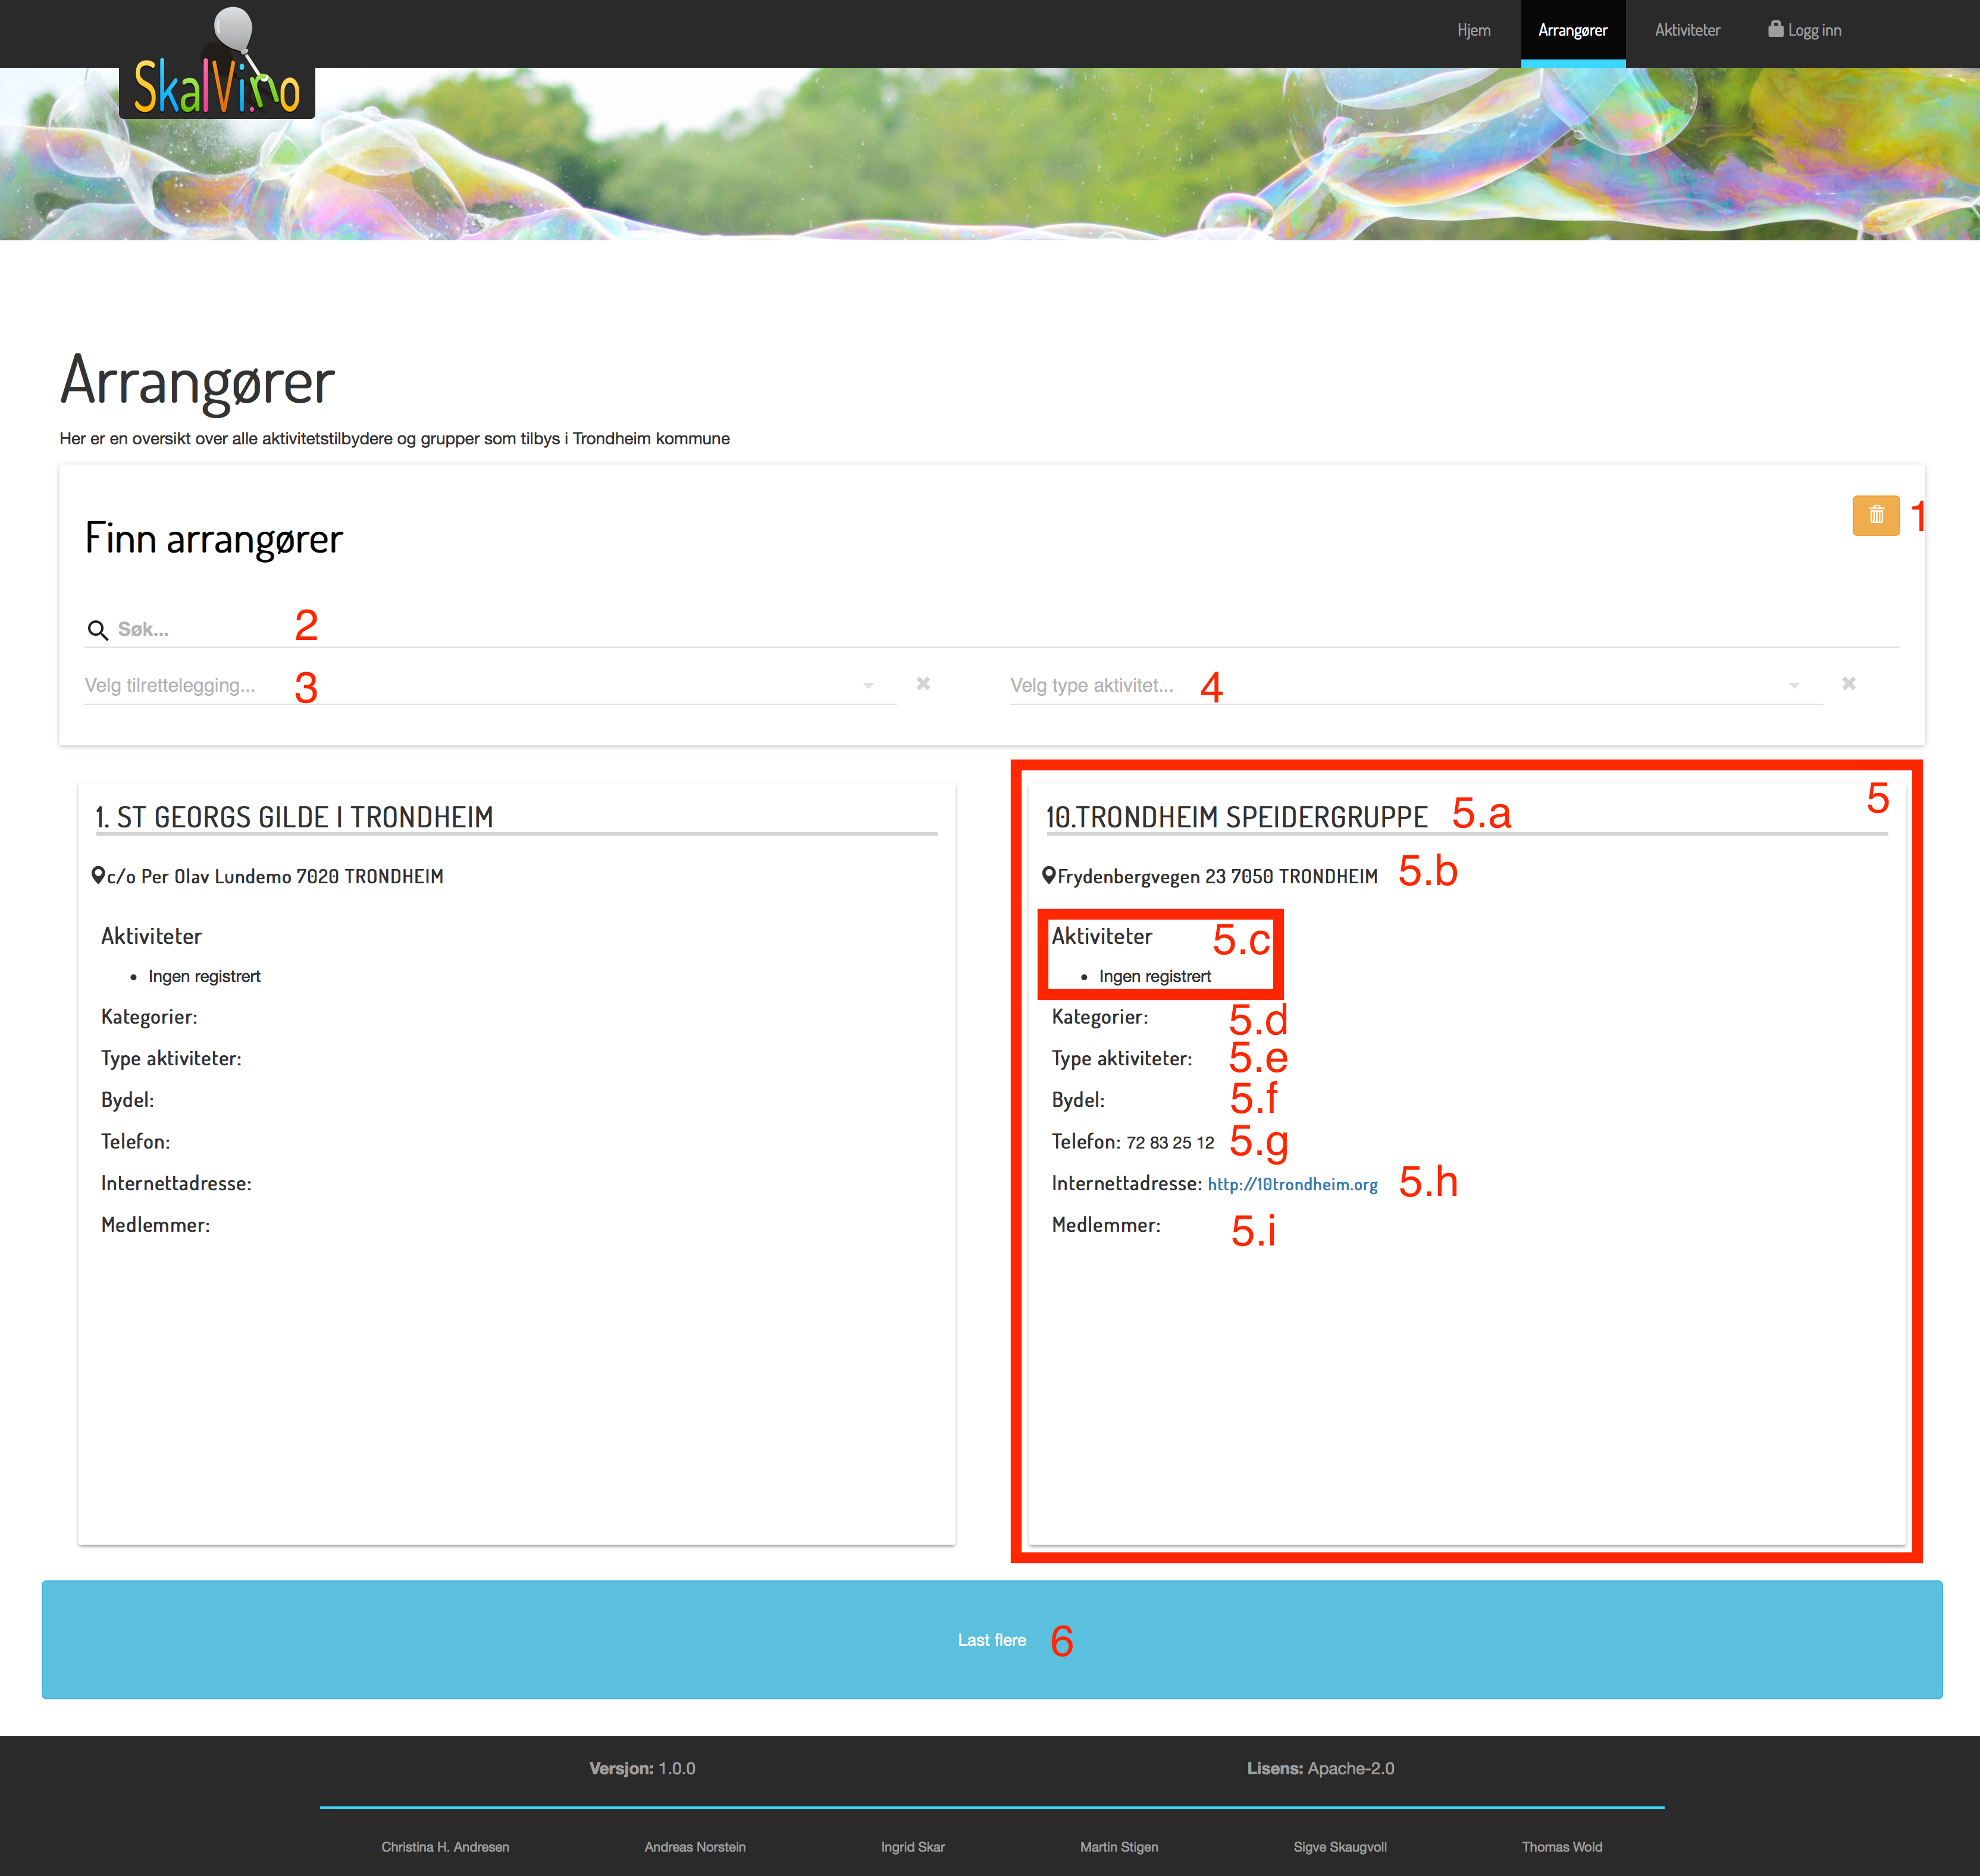
\includegraphics[height=80mm, width=\paperwidth-15mm]{appendix/manualPictures/A-providers-cut.png}}
\end{center}
\begin{enumerate}[nosep]
    \item Knapp for å tømme og tilbakestille søke valg (punkter 2,3 og 4)
    \item Her kan man begynne å skrive navn på arrangører, også kommer det en liste med arrangører som passer til innskrevet navn.
    \item Her kan man velge mellom registrerte tilrettelegginger som arrangører har registrert at de tilrettelegger for.
    \item Her kan man velge mellom registrerte typer aktiviteter man ønsker, og spesifiserer da at arrangører som vises, skal tilby aktiviteter med slik tilrettelegging.
    \item Dette er en flis, som inneholder informasjon registrert i Aktørdatabase til Trondheim Kommune om en registrert arrangør. Når siden lastes førstegang, vises det 10 arrangører.
    \begin{enumerate}
        \item Navn på arrangør.
        \item Adresse til arrangør.
        \item Hver vil aktiviteter som er laget på vegne av arrangøren vises i en liste.
        \item Hvilken kategorier arrangøren er registrert som.
        \item Hvilken type aktiviteter arrangøren registrerer.
        \item Hvilken bydel arrangøren tilhører.
        \item Telefon nummer til arrangør.
        \item Hjemmesiden / nettstedet til arrangøren.
        \item Hvor mange registrerte medlemmer arrangøren har.
    \end{enumerate}
    \item Trykk her for å laste inn 50 andre registrerte arrangører. Laster inn og viser 50 nye arrangører hver gang. Viser nye sammen med tidligere lastet. 
\end{enumerate}

\subsection{Aktiviteter}
\begin{center}
  \makebox[\textwidth]{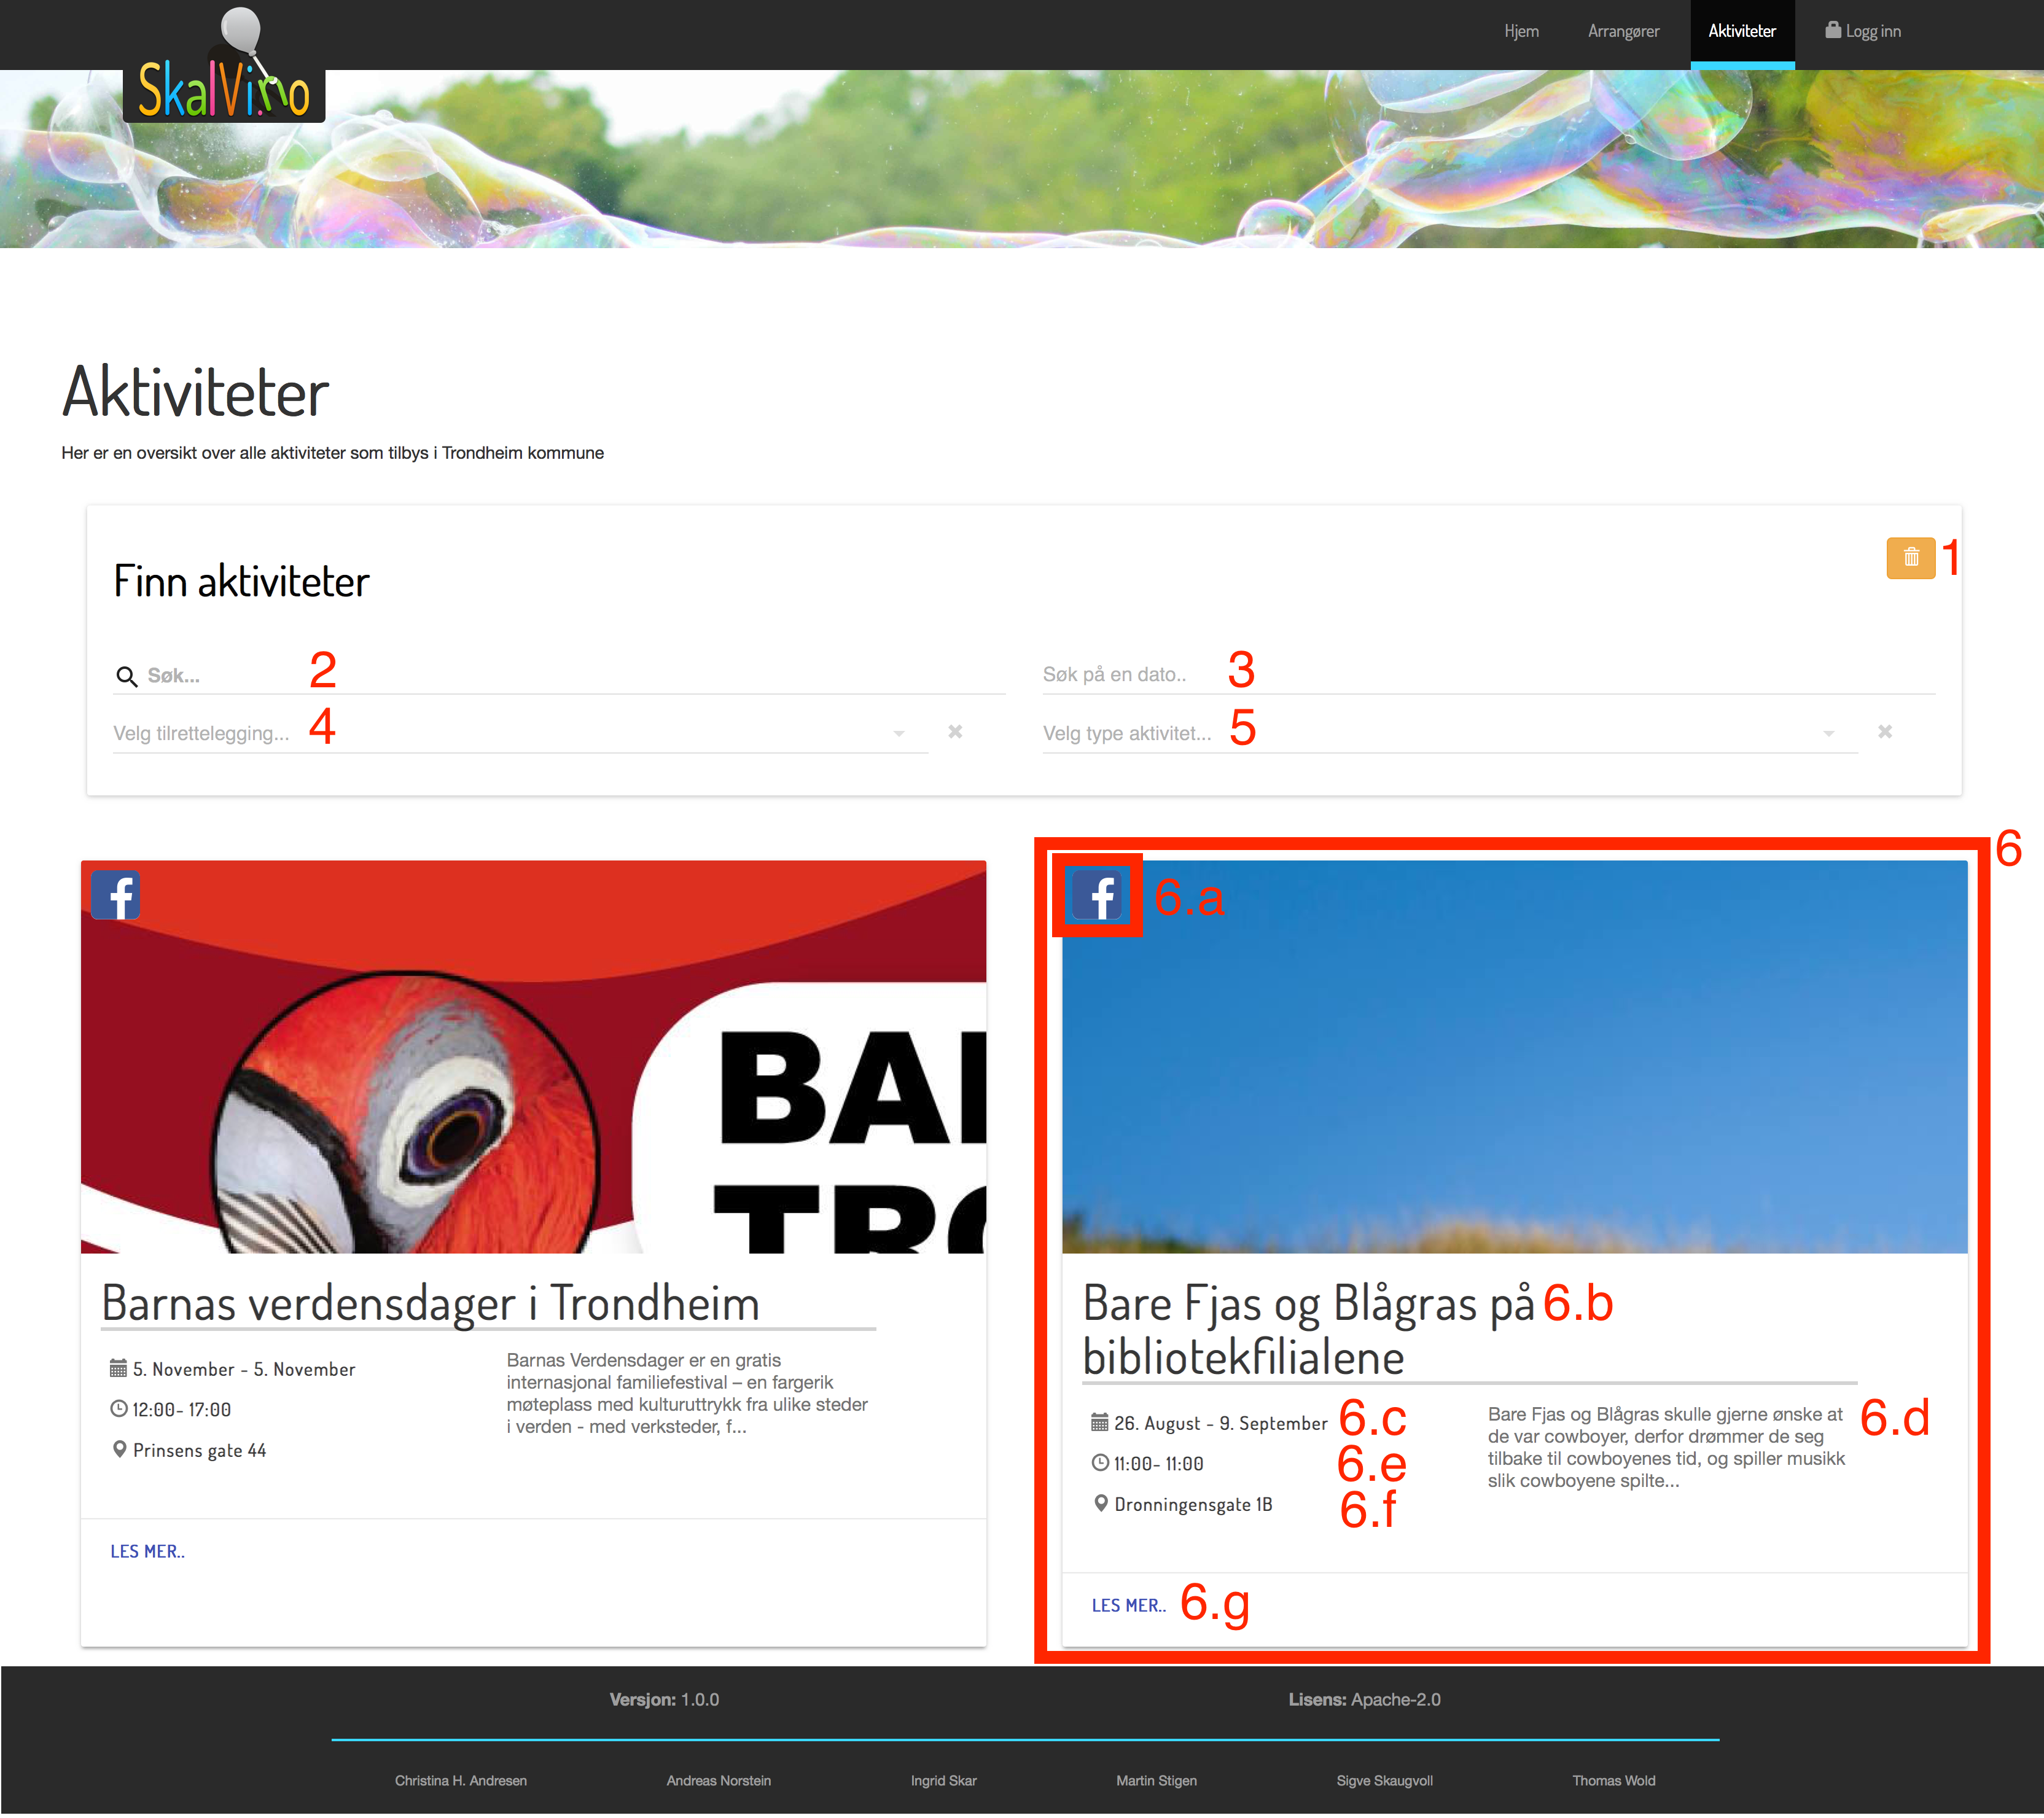
\includegraphics[height=80mm, width=\paperwidth-15mm]{appendix/manualPictures/A-activities-cut.png}}
\end{center}
\begin{enumerate}[nosep]
    \item Knapp for å tømme og tilbakestille søke valg (punkter 2,3 og 4)
    \item Her kan man begynne å skrive navn på aktiviteter også kommer det en liste med aktiviteter som passer til innskrevet aktivitet.
    \item Her spesifiserer man fra hvilken startdato aktiviteter som skal vises må være etter.
    \item Her kan man velge mellom registrerte tilrettelegginger som arrangører har registrert at aktivitet er tilrettelagt for.
    \item Her kan man velge mellom registrerte typer aktiviteter man ønsker, og spesifiserer da at aktiviteter som vises, skal være av de typene.
    \item Denne flisen er informasjon om en registrert aktivitet. Aktivitene er sortert etter startdato. Flisen kan trykkes på får å få mer informasjon åpner modal (se: modal).
    \begin{enumerate}
        \item Dette ikonet viser at aktiviteten er basert på et Facebook arrangement, og hvis man trykker på ikonet, blir man tatt til arrangementet på Facebook.
        \item Navn på aktivitet
        \item Spesifiserer hvilken periode aktiviteten pågår. 
        \item Kort introduksjon til hva aktiviteten er.
        \item Varigheten til aktiviteten
        \item Adressen hvor aktiviteten skal utføres
        \item Knapp for å åpne modal med mer informasjon om aktivitet.
    \end{enumerate}
\end{enumerate}

%%%%%%%%%%%%%%%%%%% INNLOGGET %%%%%%%%%%%%%%%%%%%

\section{Innlogget}

\subsection{Forside}
\begin{center}
  \makebox[\textwidth]{\includegraphics[height=80mm, width=\paperwidth-15mm]{appendix/manualPictures/S-home-cut.png}}
\end{center}
\begin{enumerate}[nosep]
    \item Når man er logget inn, ser navigasjonsbaren litt annerledes ut. Den har to nye sider. En for å opprette ny aktivitet (se: ny aktivitet) og en som gir deg tilgang til dit personlige innhold
    \item Disse alternativene er bare synlige når man har trykket på brukernavnet under punkt 1.
    \begin{enumerate}
        \item Trykk her for å komme til din personlige side.
        \item Trykk her for å bytte til en annen bruker som er registrert under familiebrukeren
        \item Trykk her for å logge ut
    \end{enumerate}
    \item Her viser de 4 neste aktivitetene du har trykket delta på. Disse er sortert etter startdato
    \begin{enumerate}
        \item Trykk på flisen for å få mer informasjon (se: modal)
    \end{enumerate}
\end{enumerate}

\subsection{Modal}
\begin{center}
  \makebox[\textwidth]{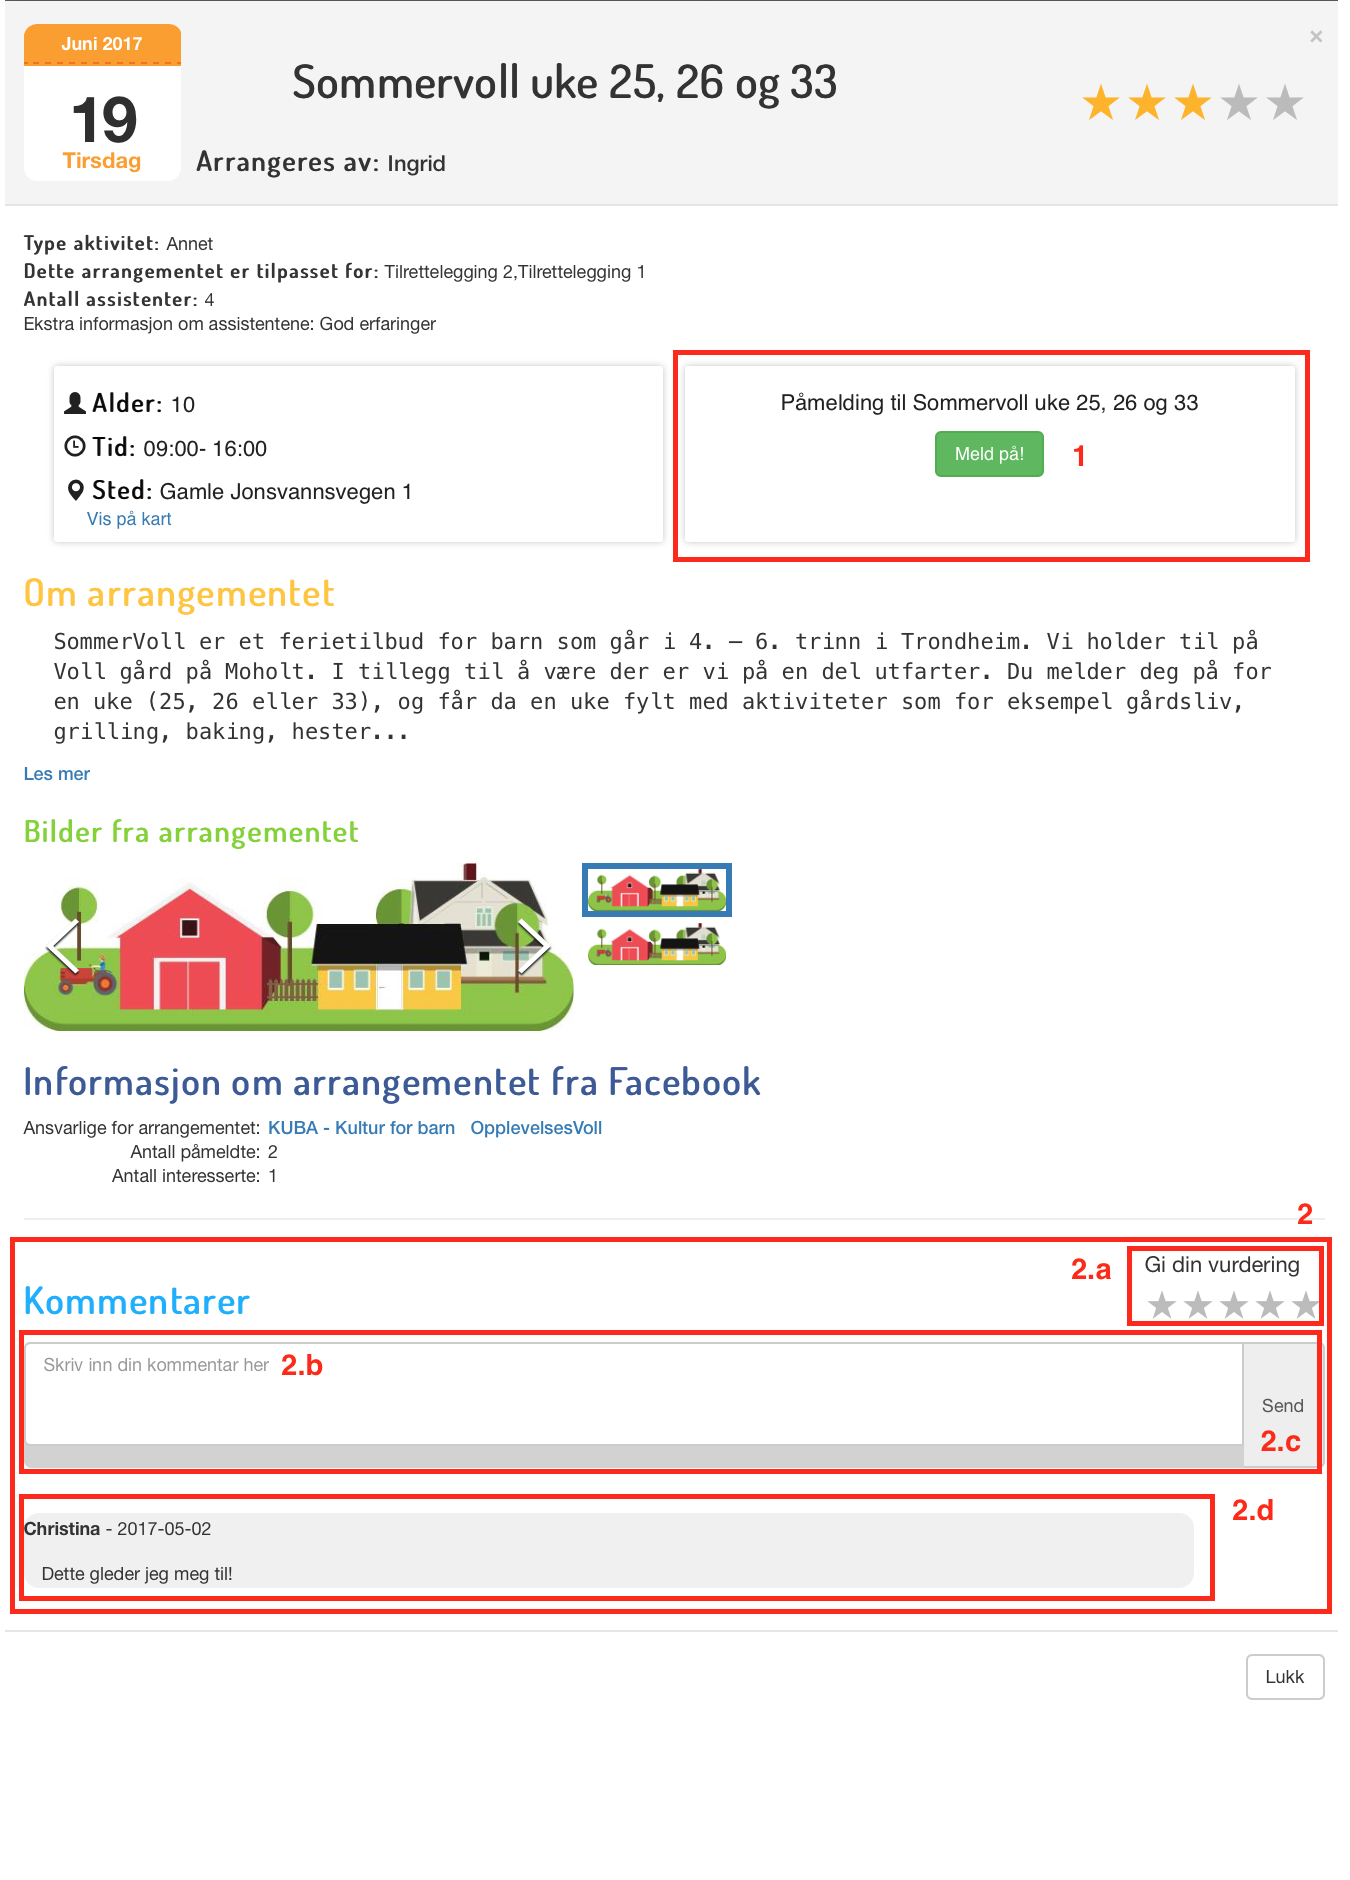
\includegraphics[height=130mm, width=\paperwidth-15mm]{appendix/manualPictures/S-modal-loggedIn-cut.png}}
\end{center}
Det er få endringer på modalen, når man er logget inn, det er litt mer funksjonalitet, men informasjonen er den samme.
\begin{enumerate}[nosep]
    \item Knapp for å melde profilen på aktiviteten og dermed kunne se den under ”Påmeldte aktiviteter” (se: ”forside” og ”min side”).
    \item Tilbakemelding på aktivitet
    \begin{enumerate}
        \item Trykk på en stjerne fra venstre til høyre for å gi en rangering til aktiviteten. Stjernen til venstre er lavest, og stjernen til høyre er best rangering.
        \item Felt for å fylle inn en kommentar til aktiviteten. NB! Kommentaren vil være synlig for andre.
        \item Knapp for å publisere kommentaren. NB! Profilnavn vil bli synlig sammen med kommentar.
        \item Liste med kommentarer. Profilnavn og publiseringsdato vises øverst til venstre. 
    \end{enumerate}
\end{enumerate}

\subsection{Arrangører}
\begin{center}
  \makebox[\textwidth]{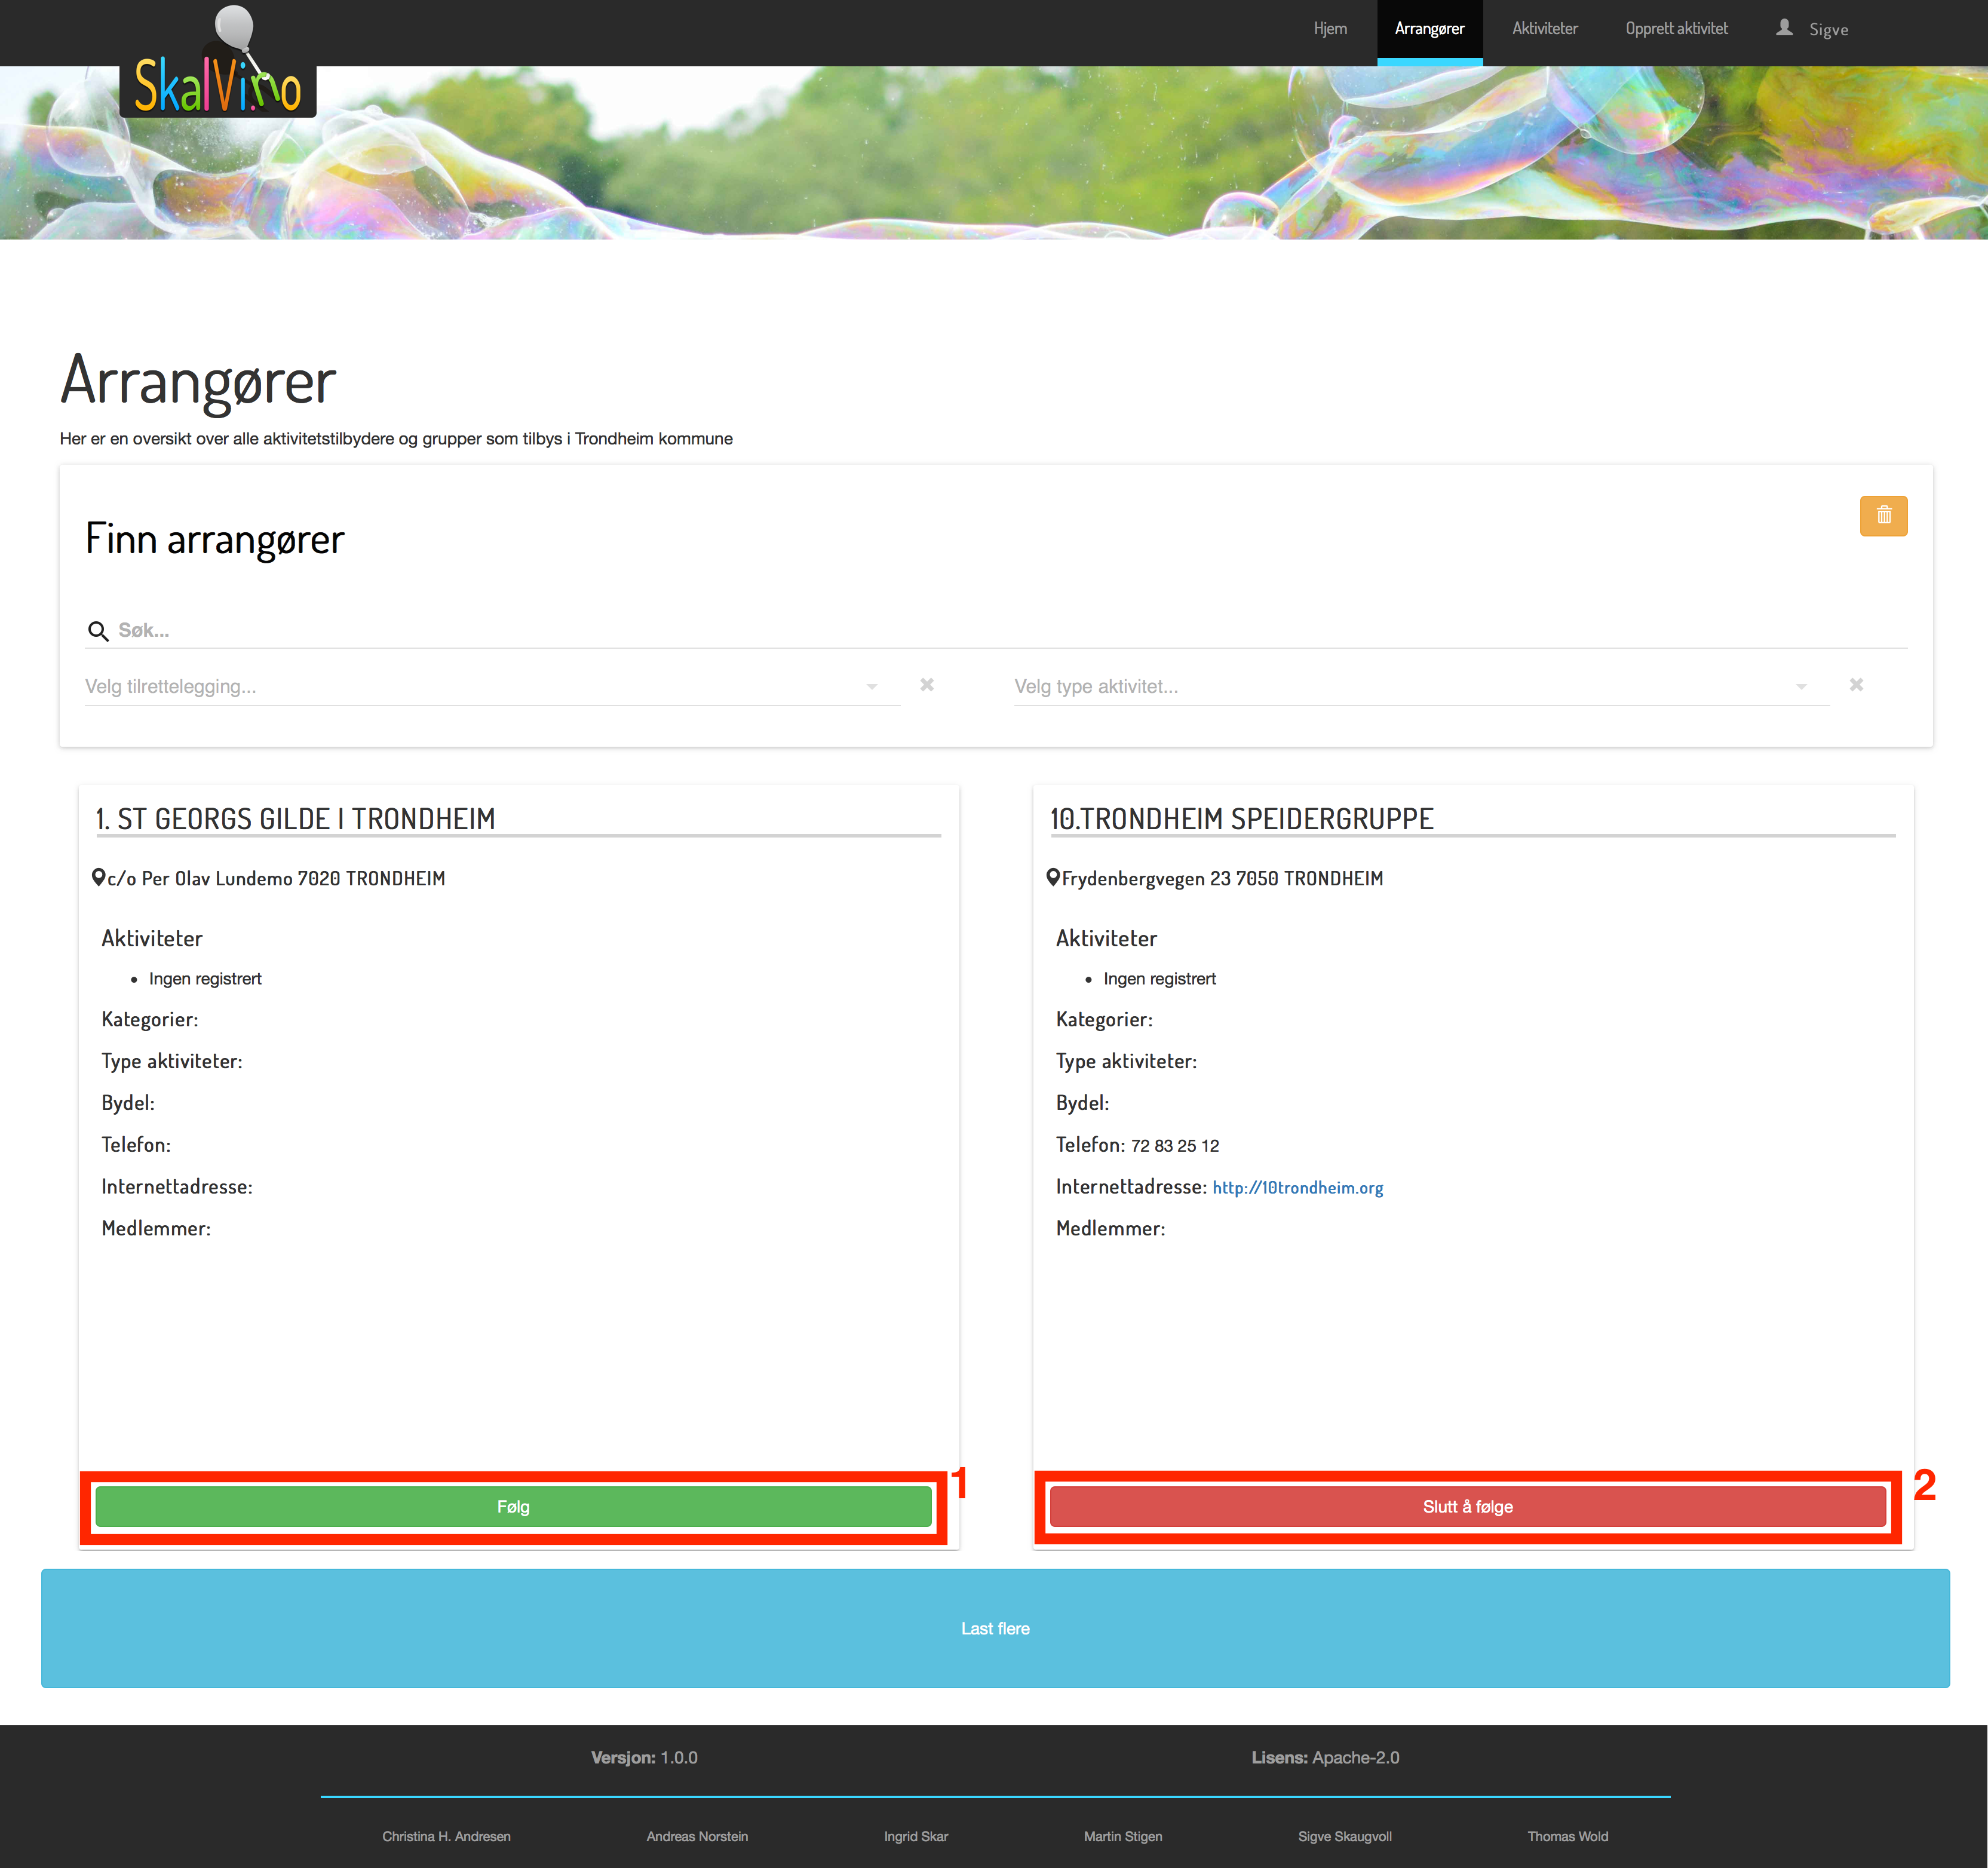
\includegraphics[height=80mm, width=\paperwidth-15mm]{appendix/manualPictures/S-providers-cut.png}}
\end{center}
\begin{enumerate}[nosep]
    \item Trykk her for å begynne å følge arrangøren.
    \item Trykk her for å slutte å følge arrangøren.
\end{enumerate}

\subsection{Ny profil}
\begin{center}
  \makebox[\textwidth]{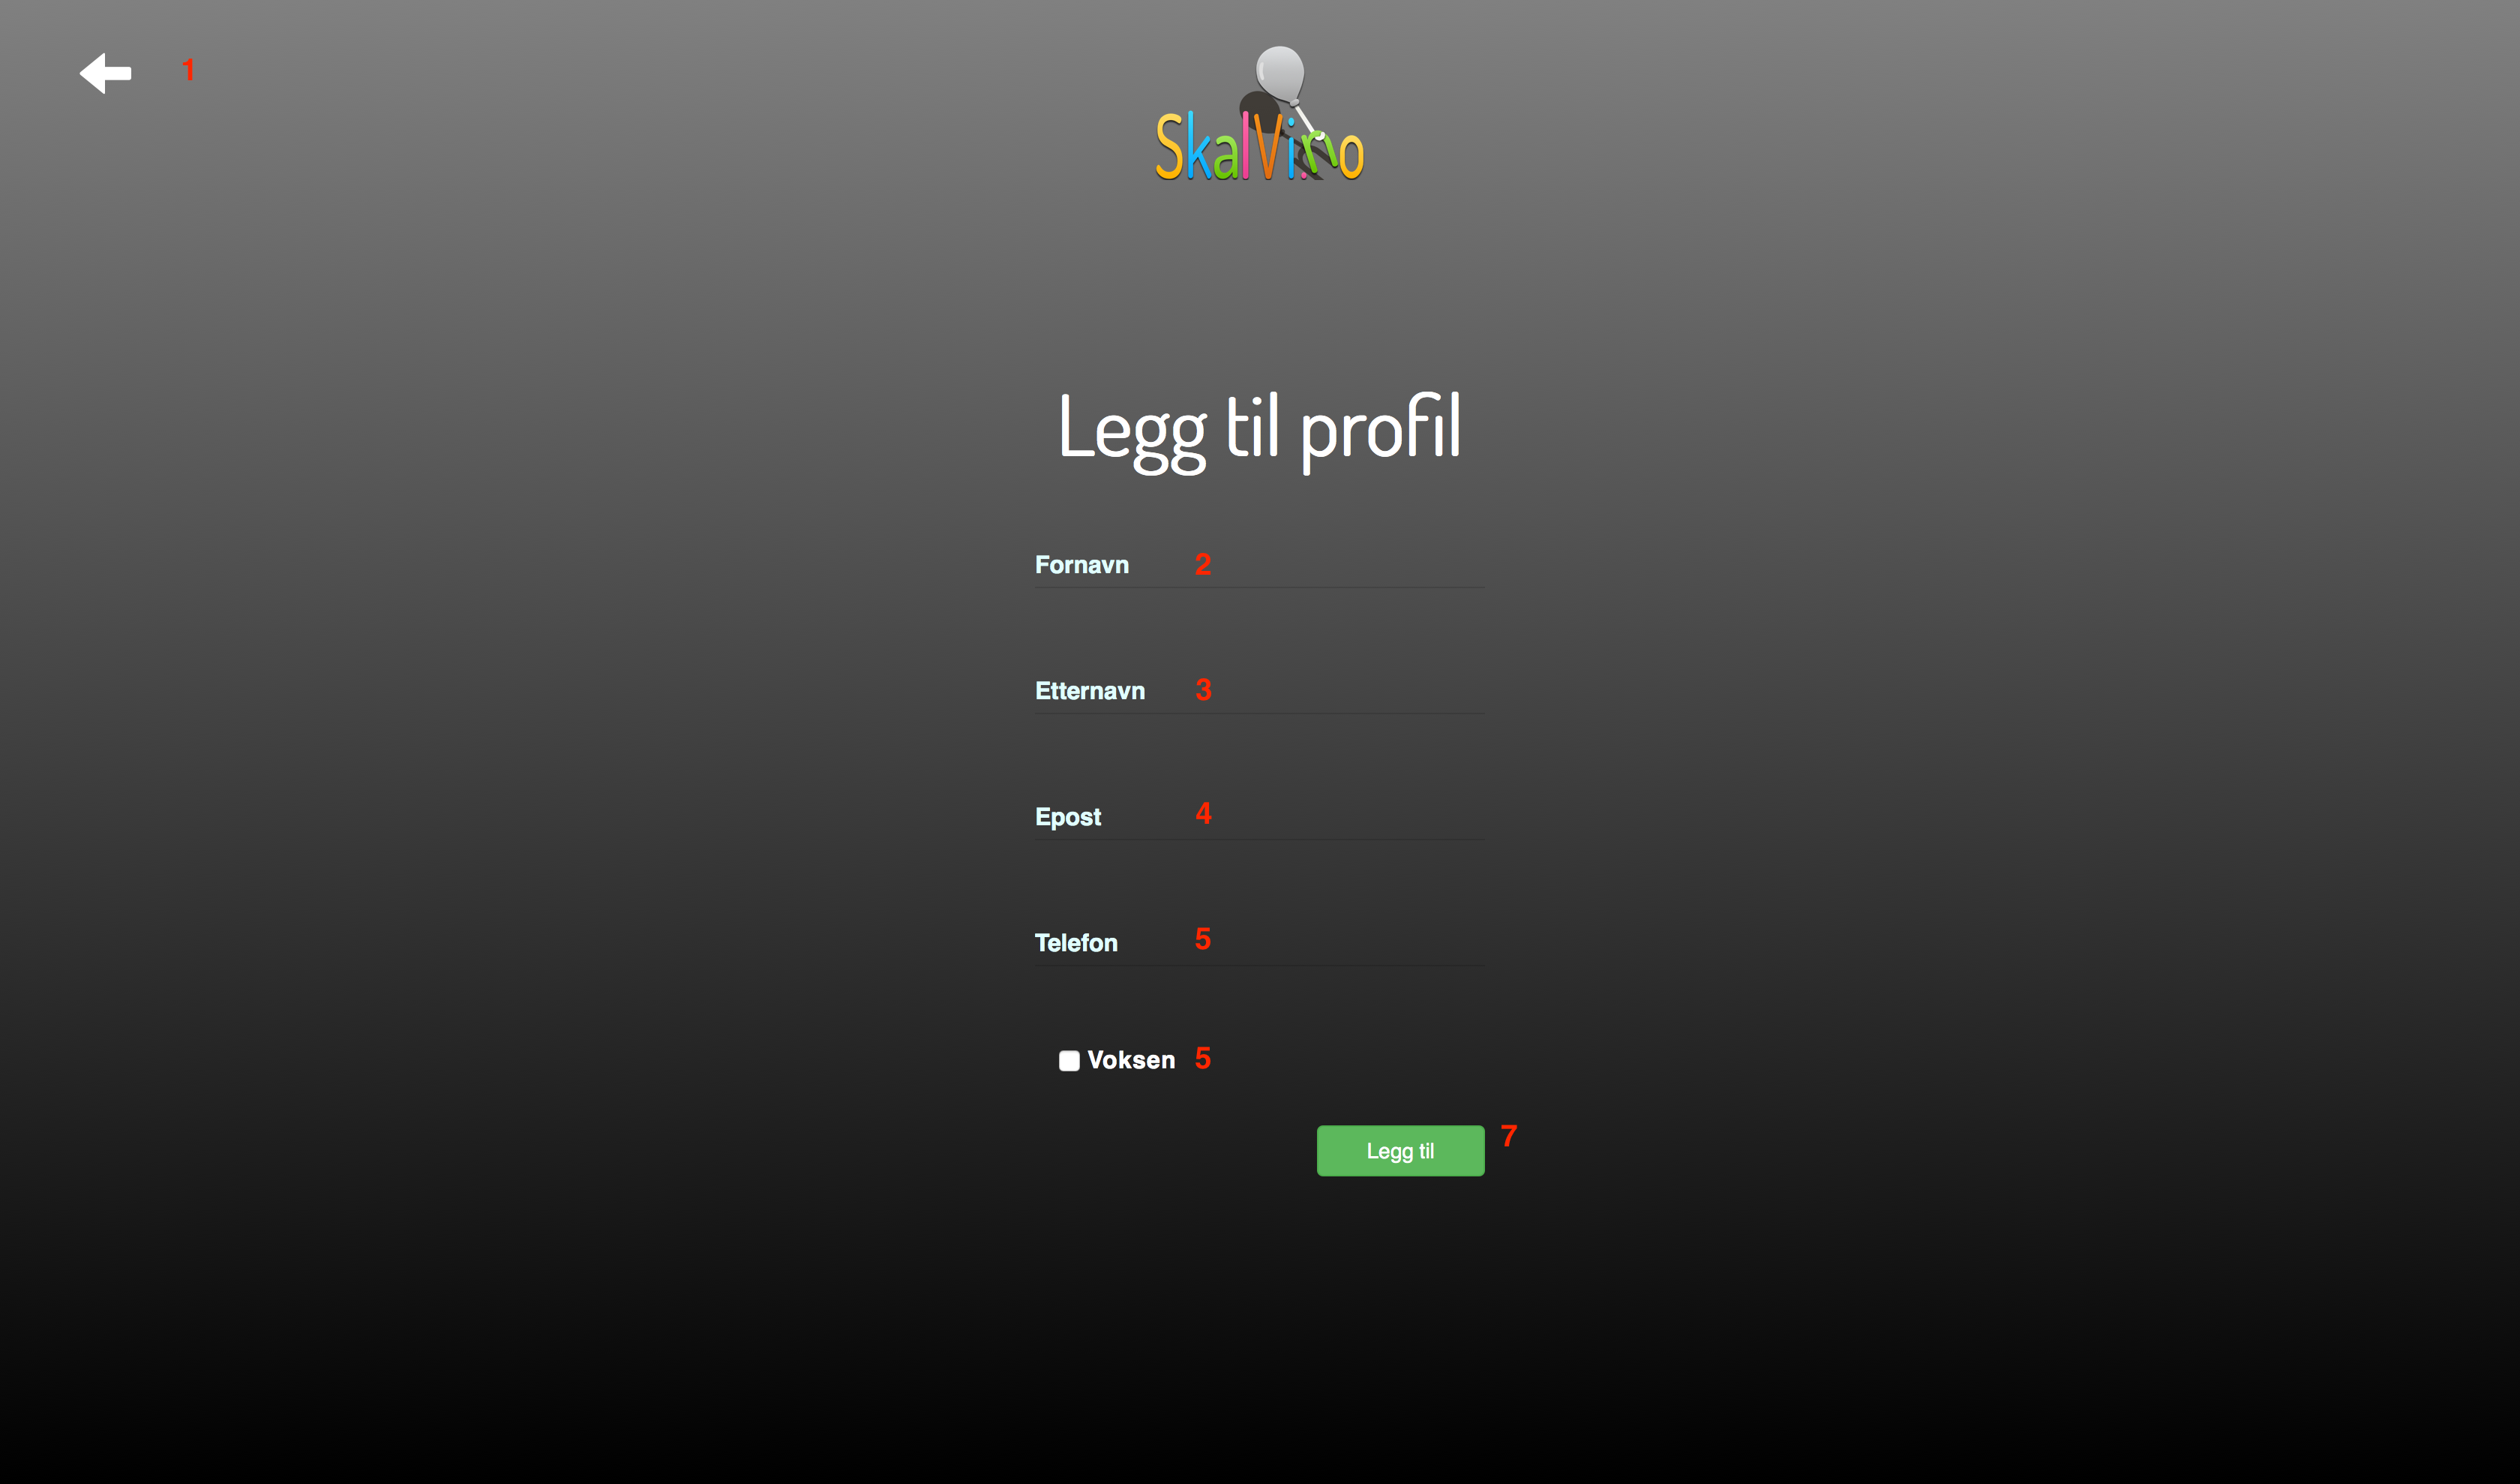
\includegraphics[height=80mm, width=\paperwidth-15mm]{appendix/manualPictures/S-addNewSubProfile-cut.png}}
\end{center}
\begin{enumerate}[nosep]
    \item Felt for å fylle inn fornavn (merk: også brukernavn) på ny underprofil
    \item Felt for å fylle inn etternavn på underprofil
    \item Felt for å fylle inn epost til underprofil
    \item Felt for å fylle inn telefonnummer til underprofil
    \item Hvis underprofil er barn / ungdom ikke trykk her. Hvis underprofil er en voksen, trykk her.
    \item Trykk her for å registrere den nye underprofilen til familiebrukeren.
\end{enumerate}

\subsection{Skifte aktiv profil}
\begin{center}
  \makebox[\textwidth]{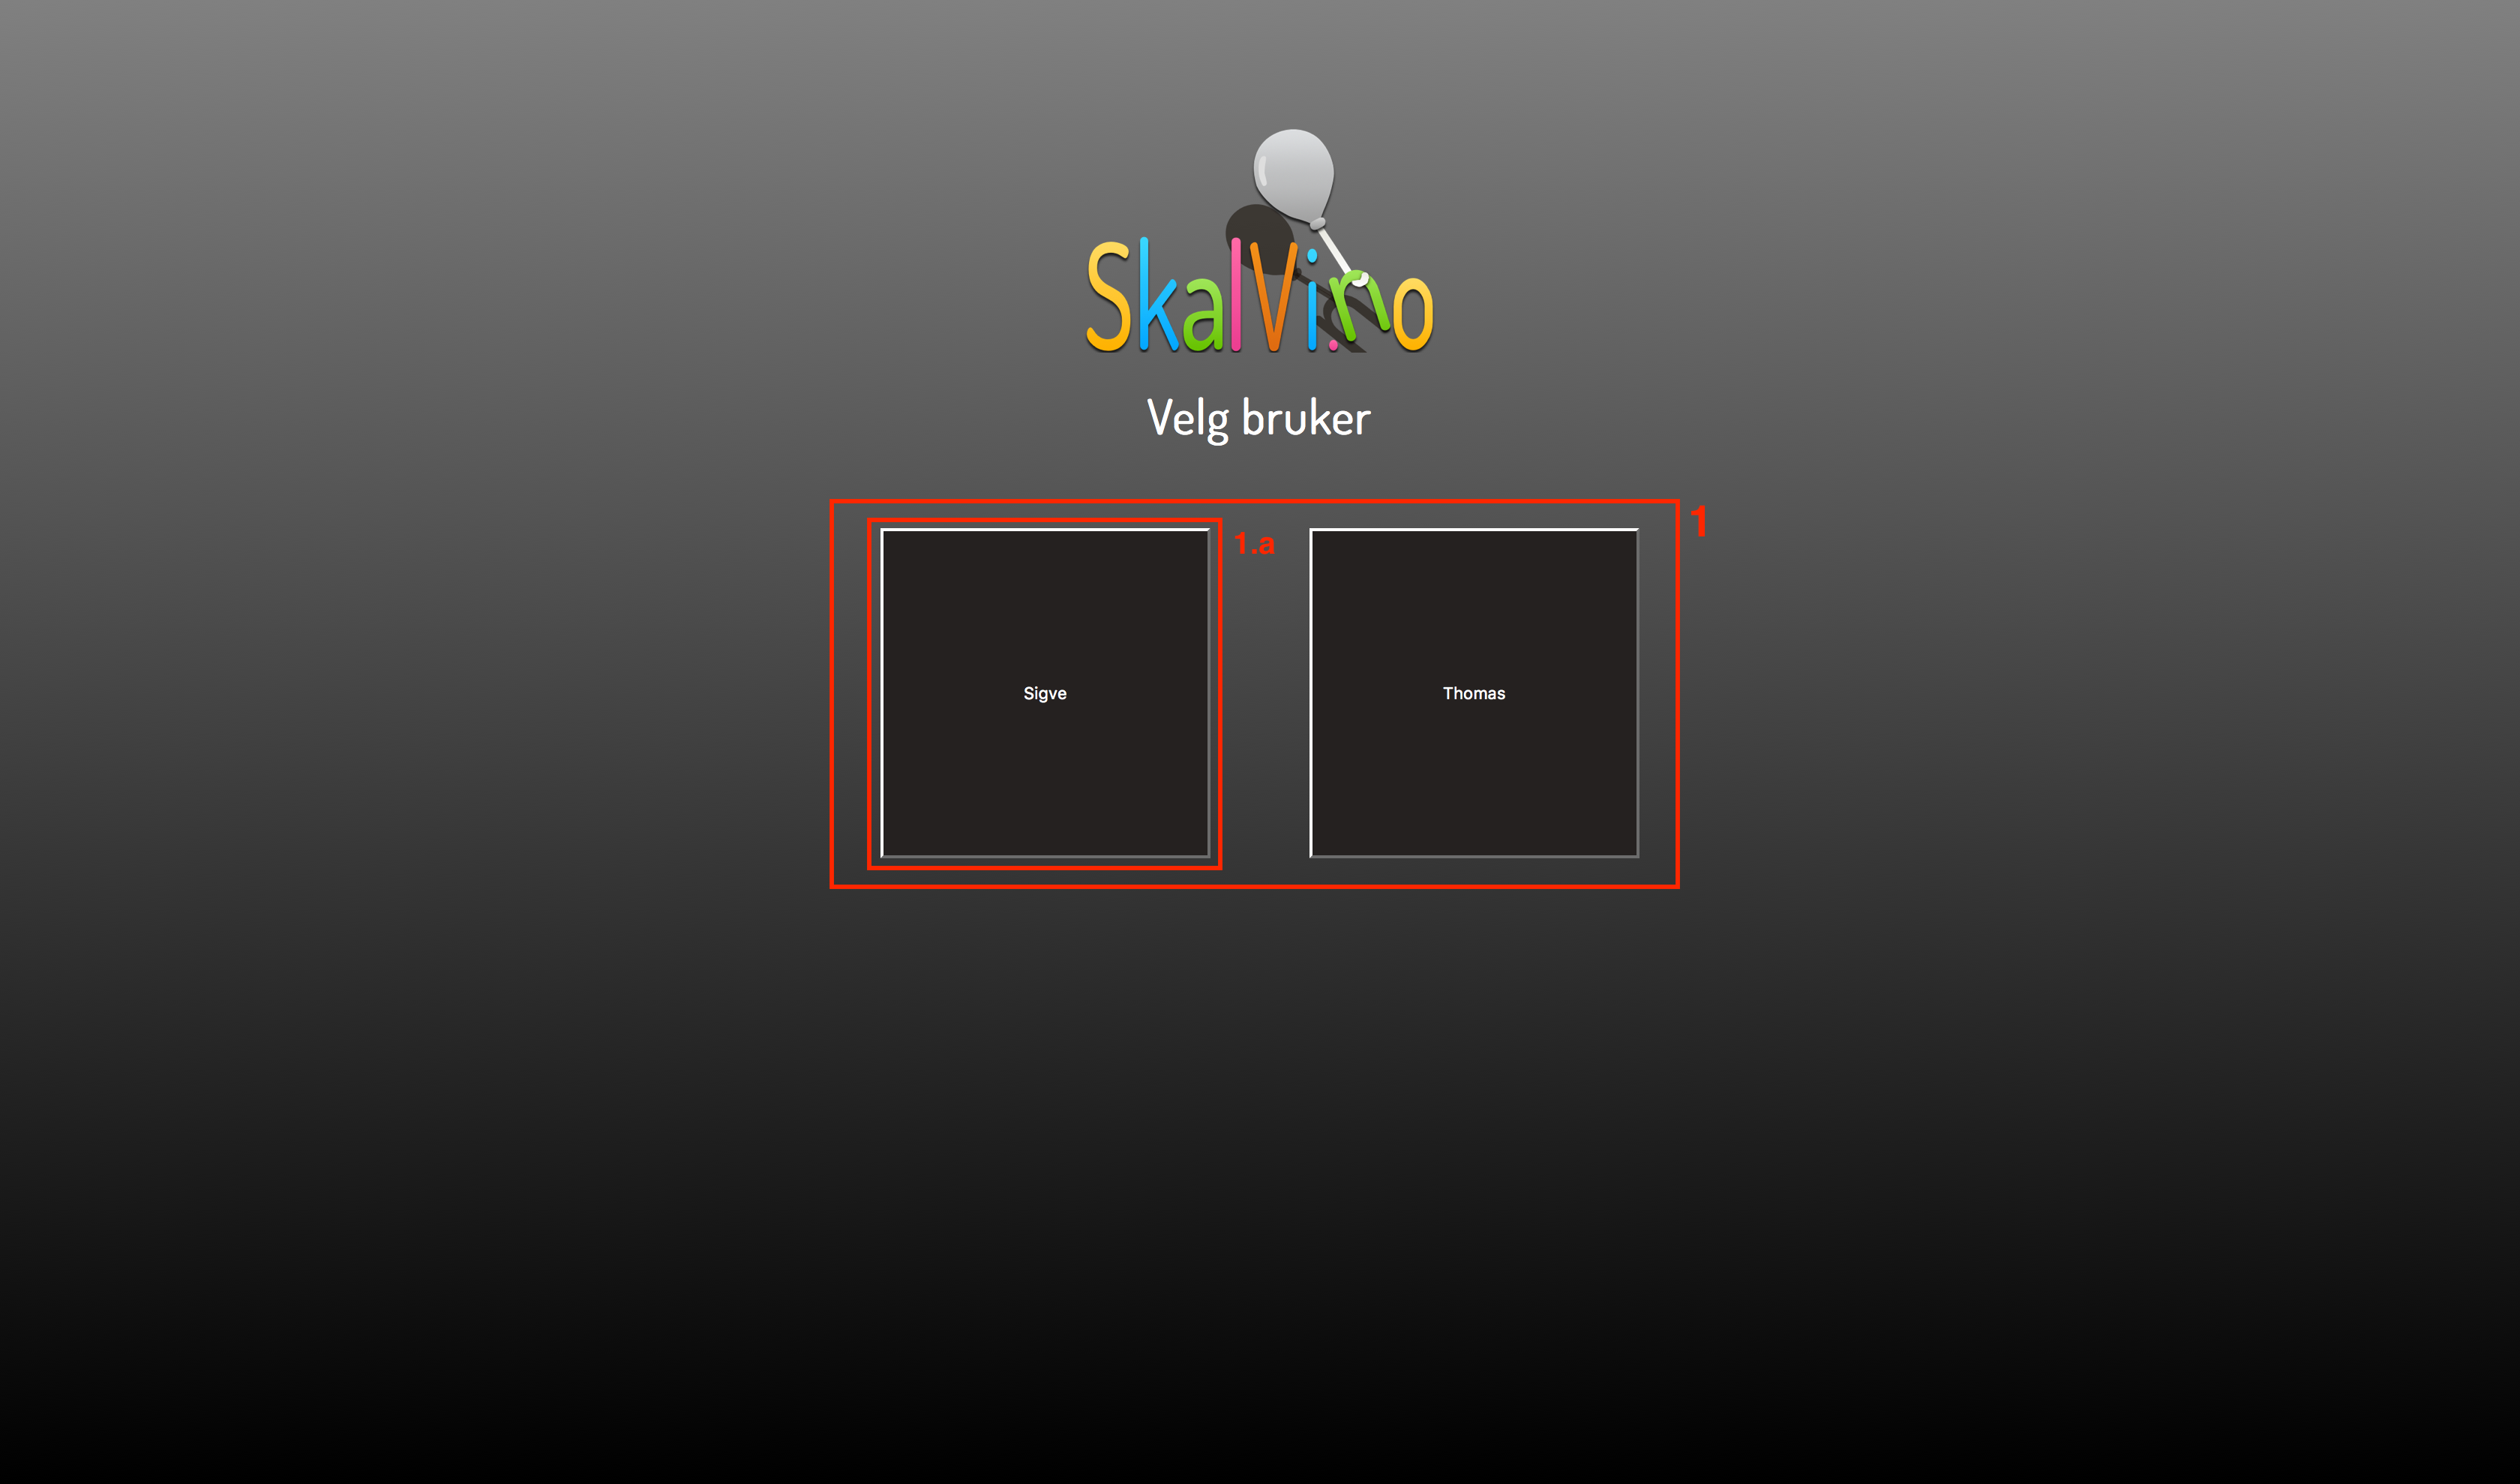
\includegraphics[height=80mm, width=\paperwidth-15mm]{appendix/manualPictures/S-changeUser-cut.png}}
\end{center}
\begin{enumerate}[nosep]
    \item Alle brukere registrert på en familiebruker, vil bli vist her i form av 1.a
    \begin{enumerate}
        \item En knapp som kan trykkes på for å velge å skifte / gjøre underprofil brukerne Sigve nåværende / aktiv bruker. 
    \end{enumerate}
\end{enumerate}

\subsection{Administrere arrangører}
\begin{center}
  \makebox[\textwidth]{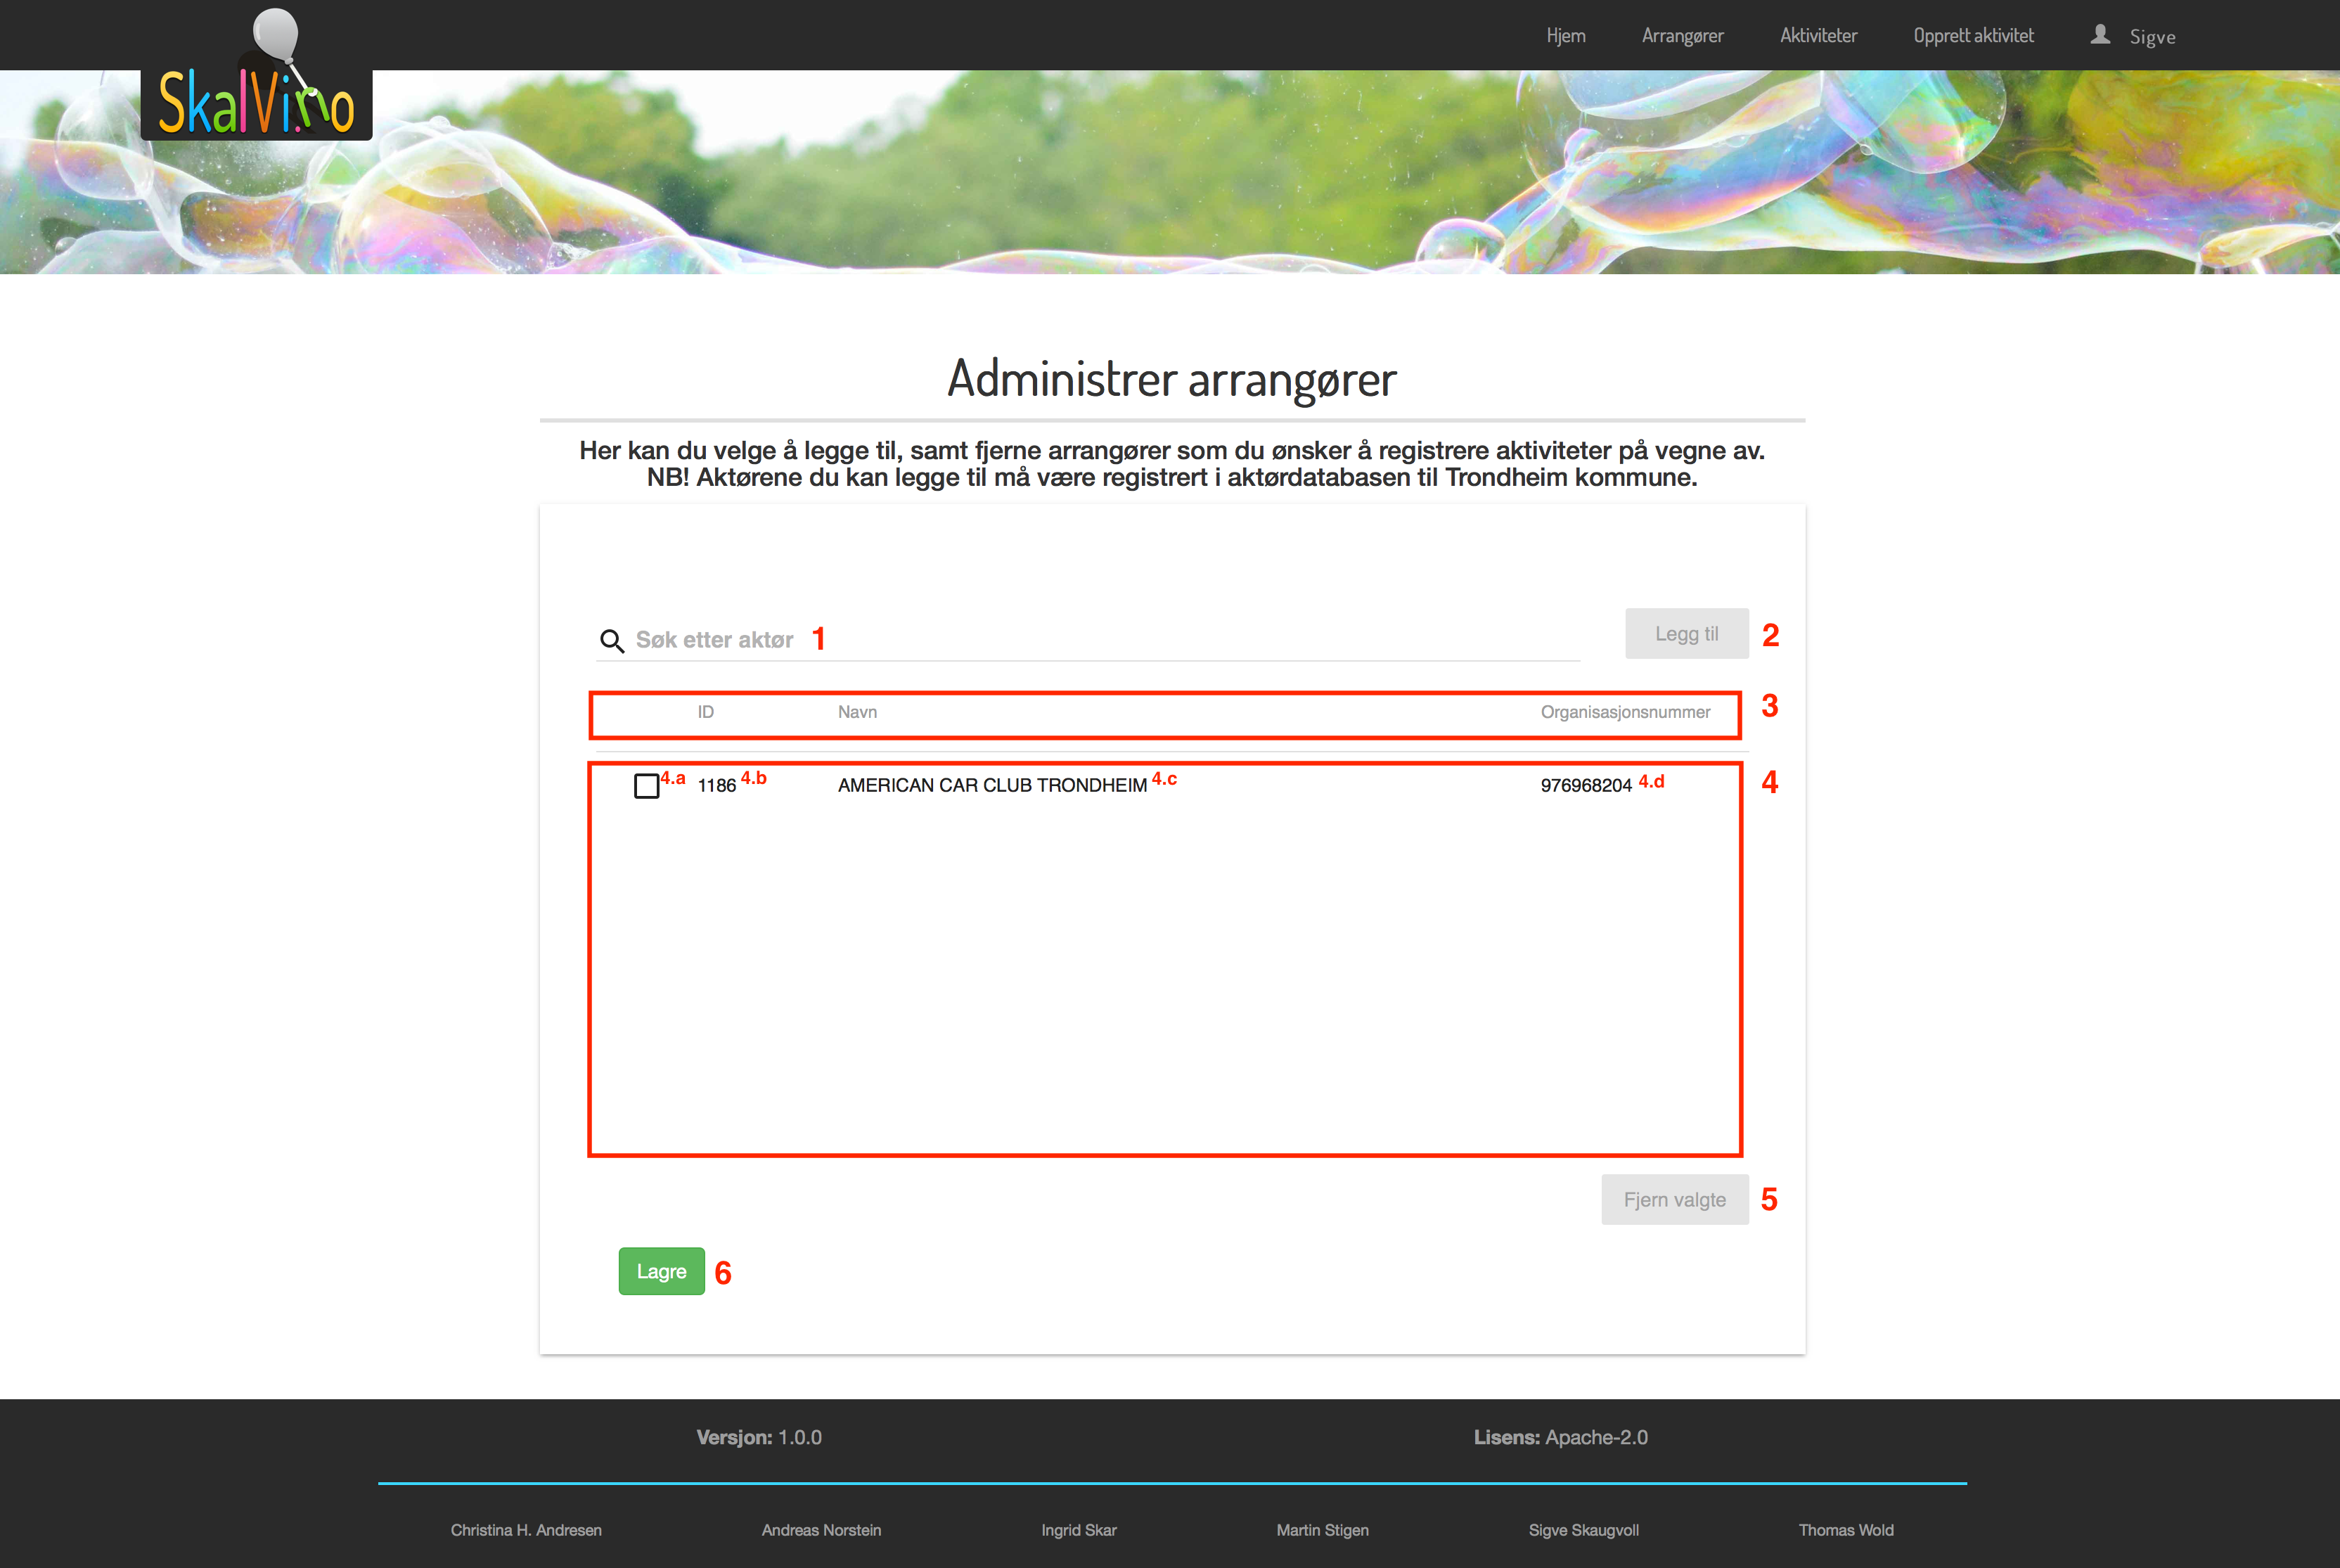
\includegraphics[height=80mm, width=\paperwidth-15mm]{appendix/manualPictures/S-addProvider-cut.png}}
\end{center}
\begin{enumerate}[nosep]
    \item Felt for å skrive navn på arrangør man ønsker å la bruke publisere aktiviteter på vegne av.
    \item Når ønsket arrangør er valgt, trykk her for å legge til arrangøren i listen (punkt 4).
    \item Beskrivelse av informasjon i punkt 4.
    \item Liste over arrangører man ønsker å kunne publisere på vegne av
    \begin{enumerate}
        \item Knapp for å velge arrangør(er)
        \item Id til arrangør i Aktørdatabasen
        \item Navn til arrangør
        \item Organisasjonsnummeret som er registrert på arrangør i Brønnøysundregisteret.
    \end{enumerate}
    \item Hvis arrangør(er) i listen (punkt 4) er valgt kan man trykke på denne for å fjerne de.
    \item Trykk her for å lagre arrangører i listen (punkt 4) til aktiv profil / bruker. 
\end{enumerate}

\subsection{Facebook login}
\begin{center}
  \makebox[\textwidth]{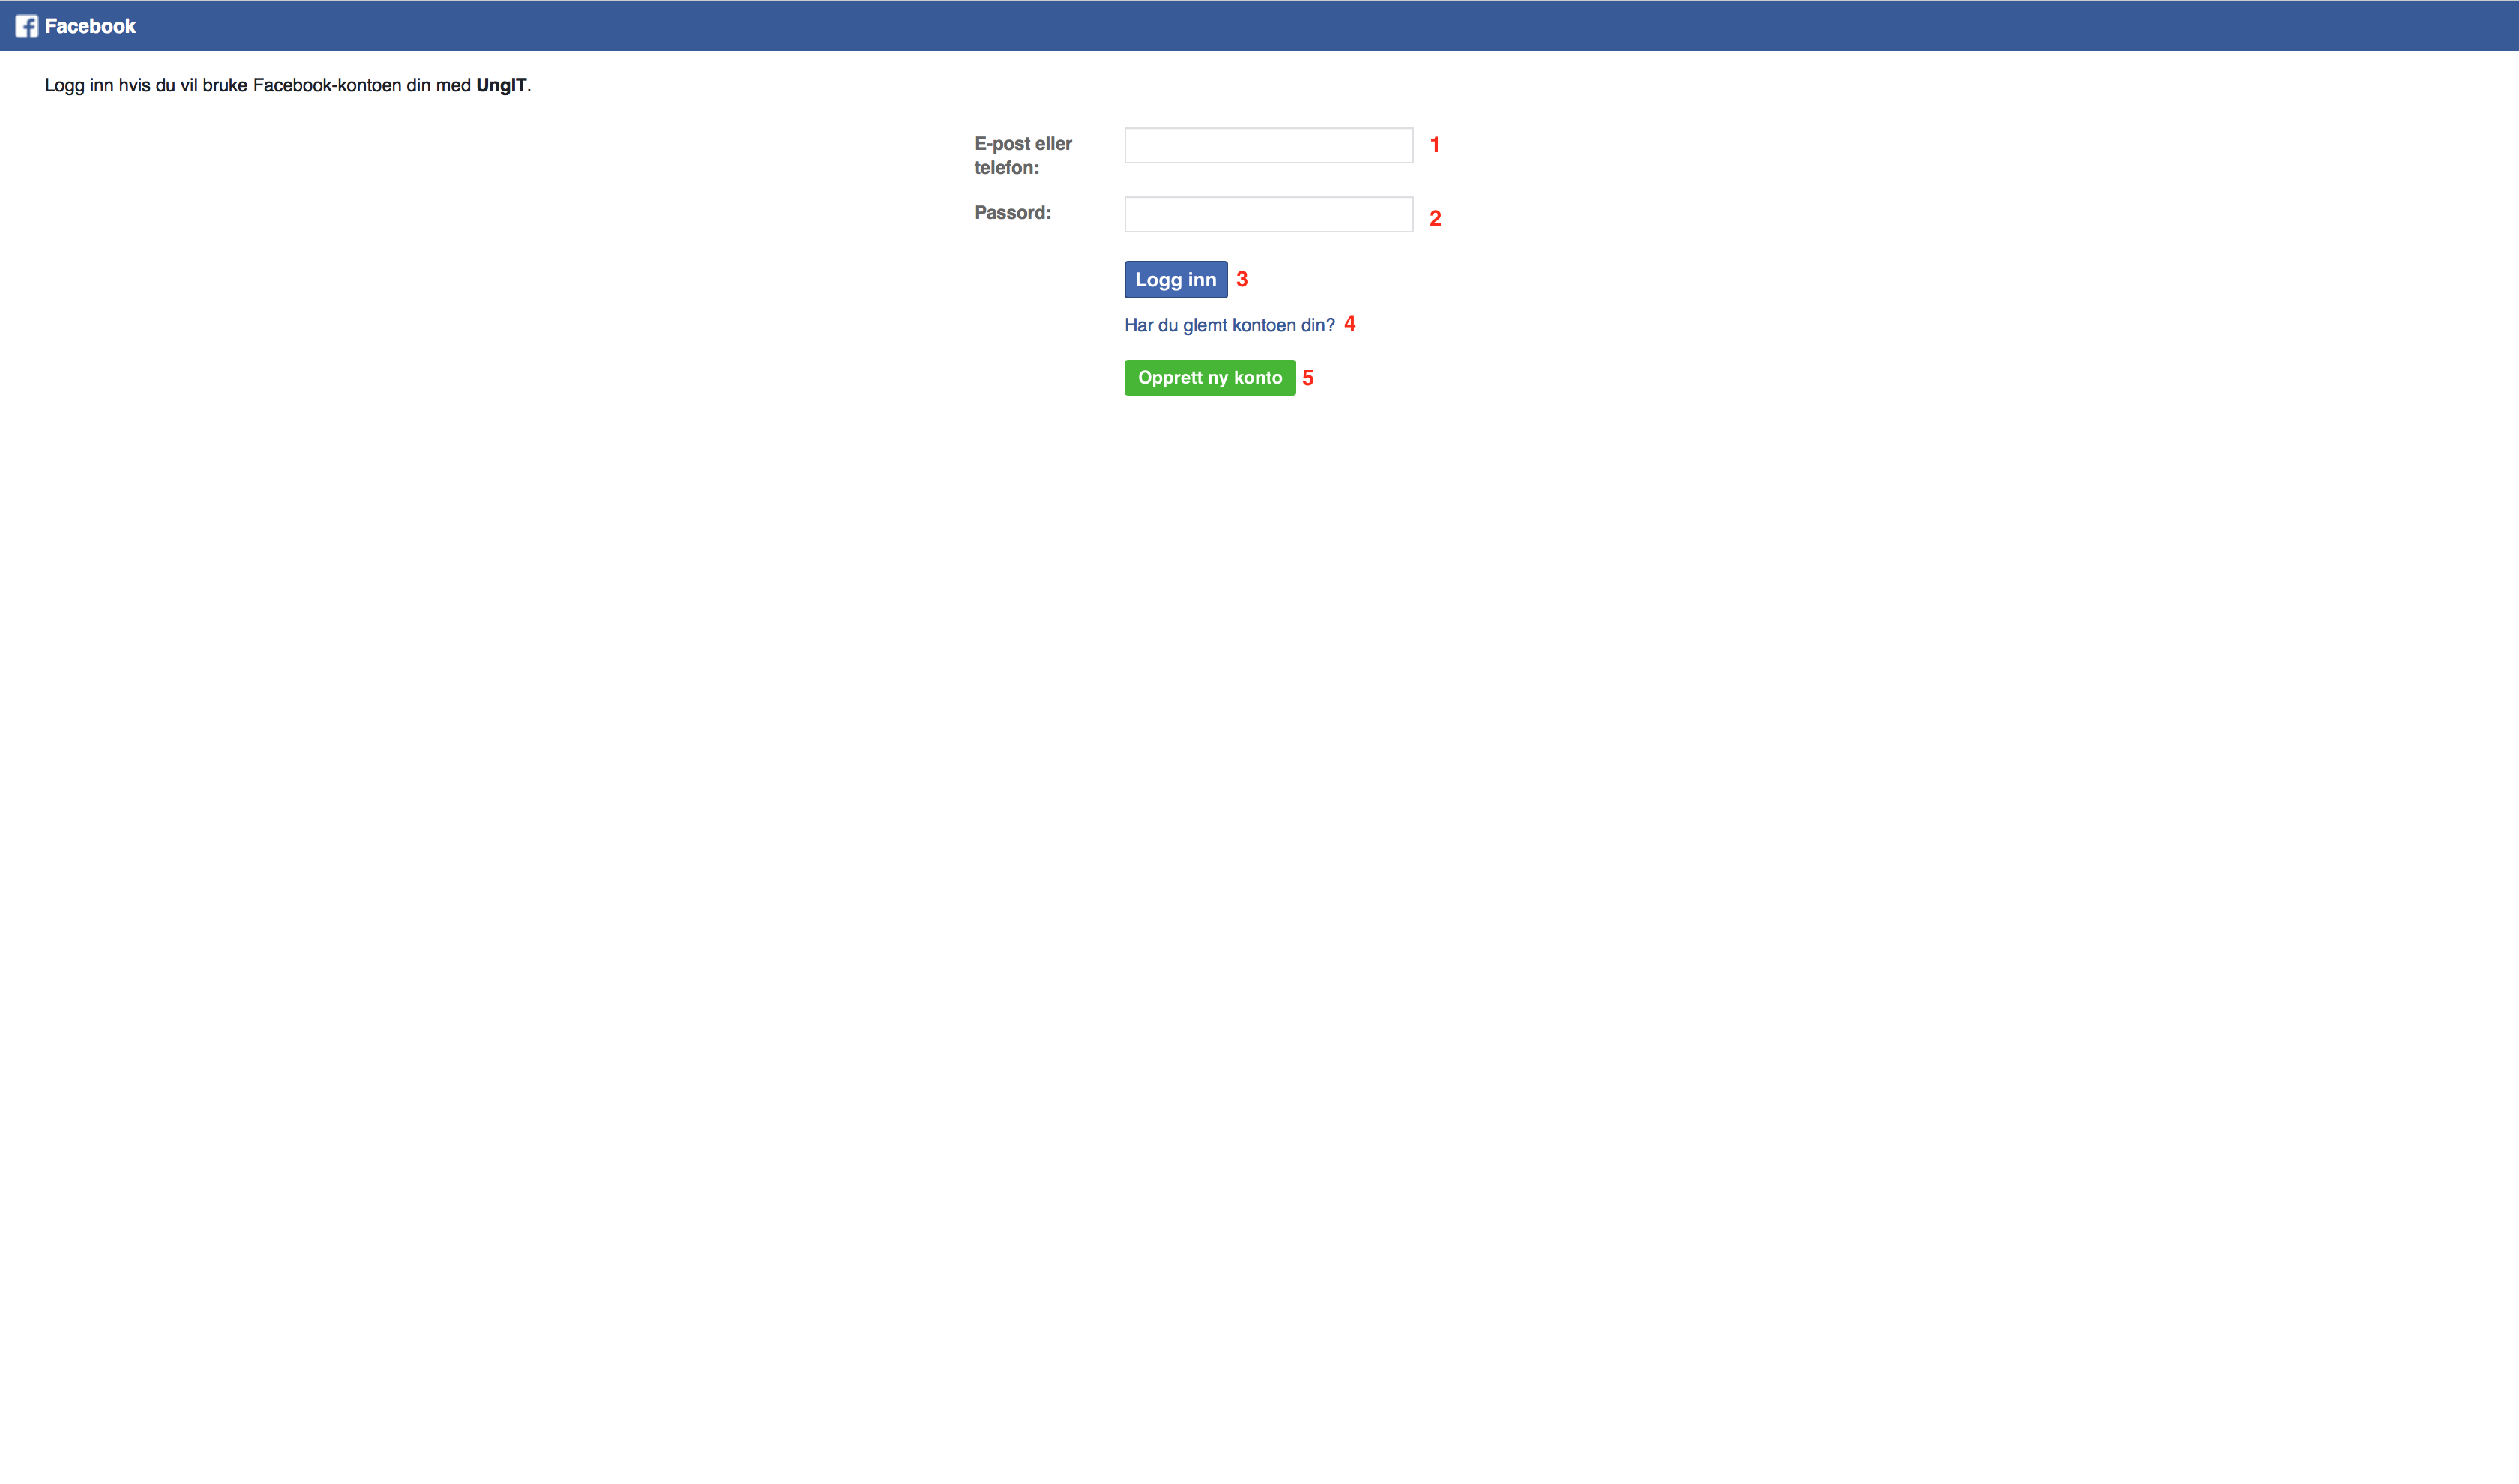
\includegraphics[height=80mm, width=\paperwidth-15mm]{appendix/manualPictures/S-Facebook-login-cut.png}}
\end{center}
NB! Denne siden er under domentet skalvi.no, men Facebook.com
\begin{enumerate}[nosep]
    \item Skriv inn epost / mobilnummer til Facebookkonto
    \item Skriv inn passord til Facebook konto
    \item Trykk her for å logge inn når punkt 1 og 2 er fylt inn.
    \item Trykk her for å få hjelp til å huske Facebook passord
    \item Trykk her hvis du ikke har Facebook konto.
\end{enumerate}

\subsection{Min Side}
\begin{center}
  \makebox[\textwidth]{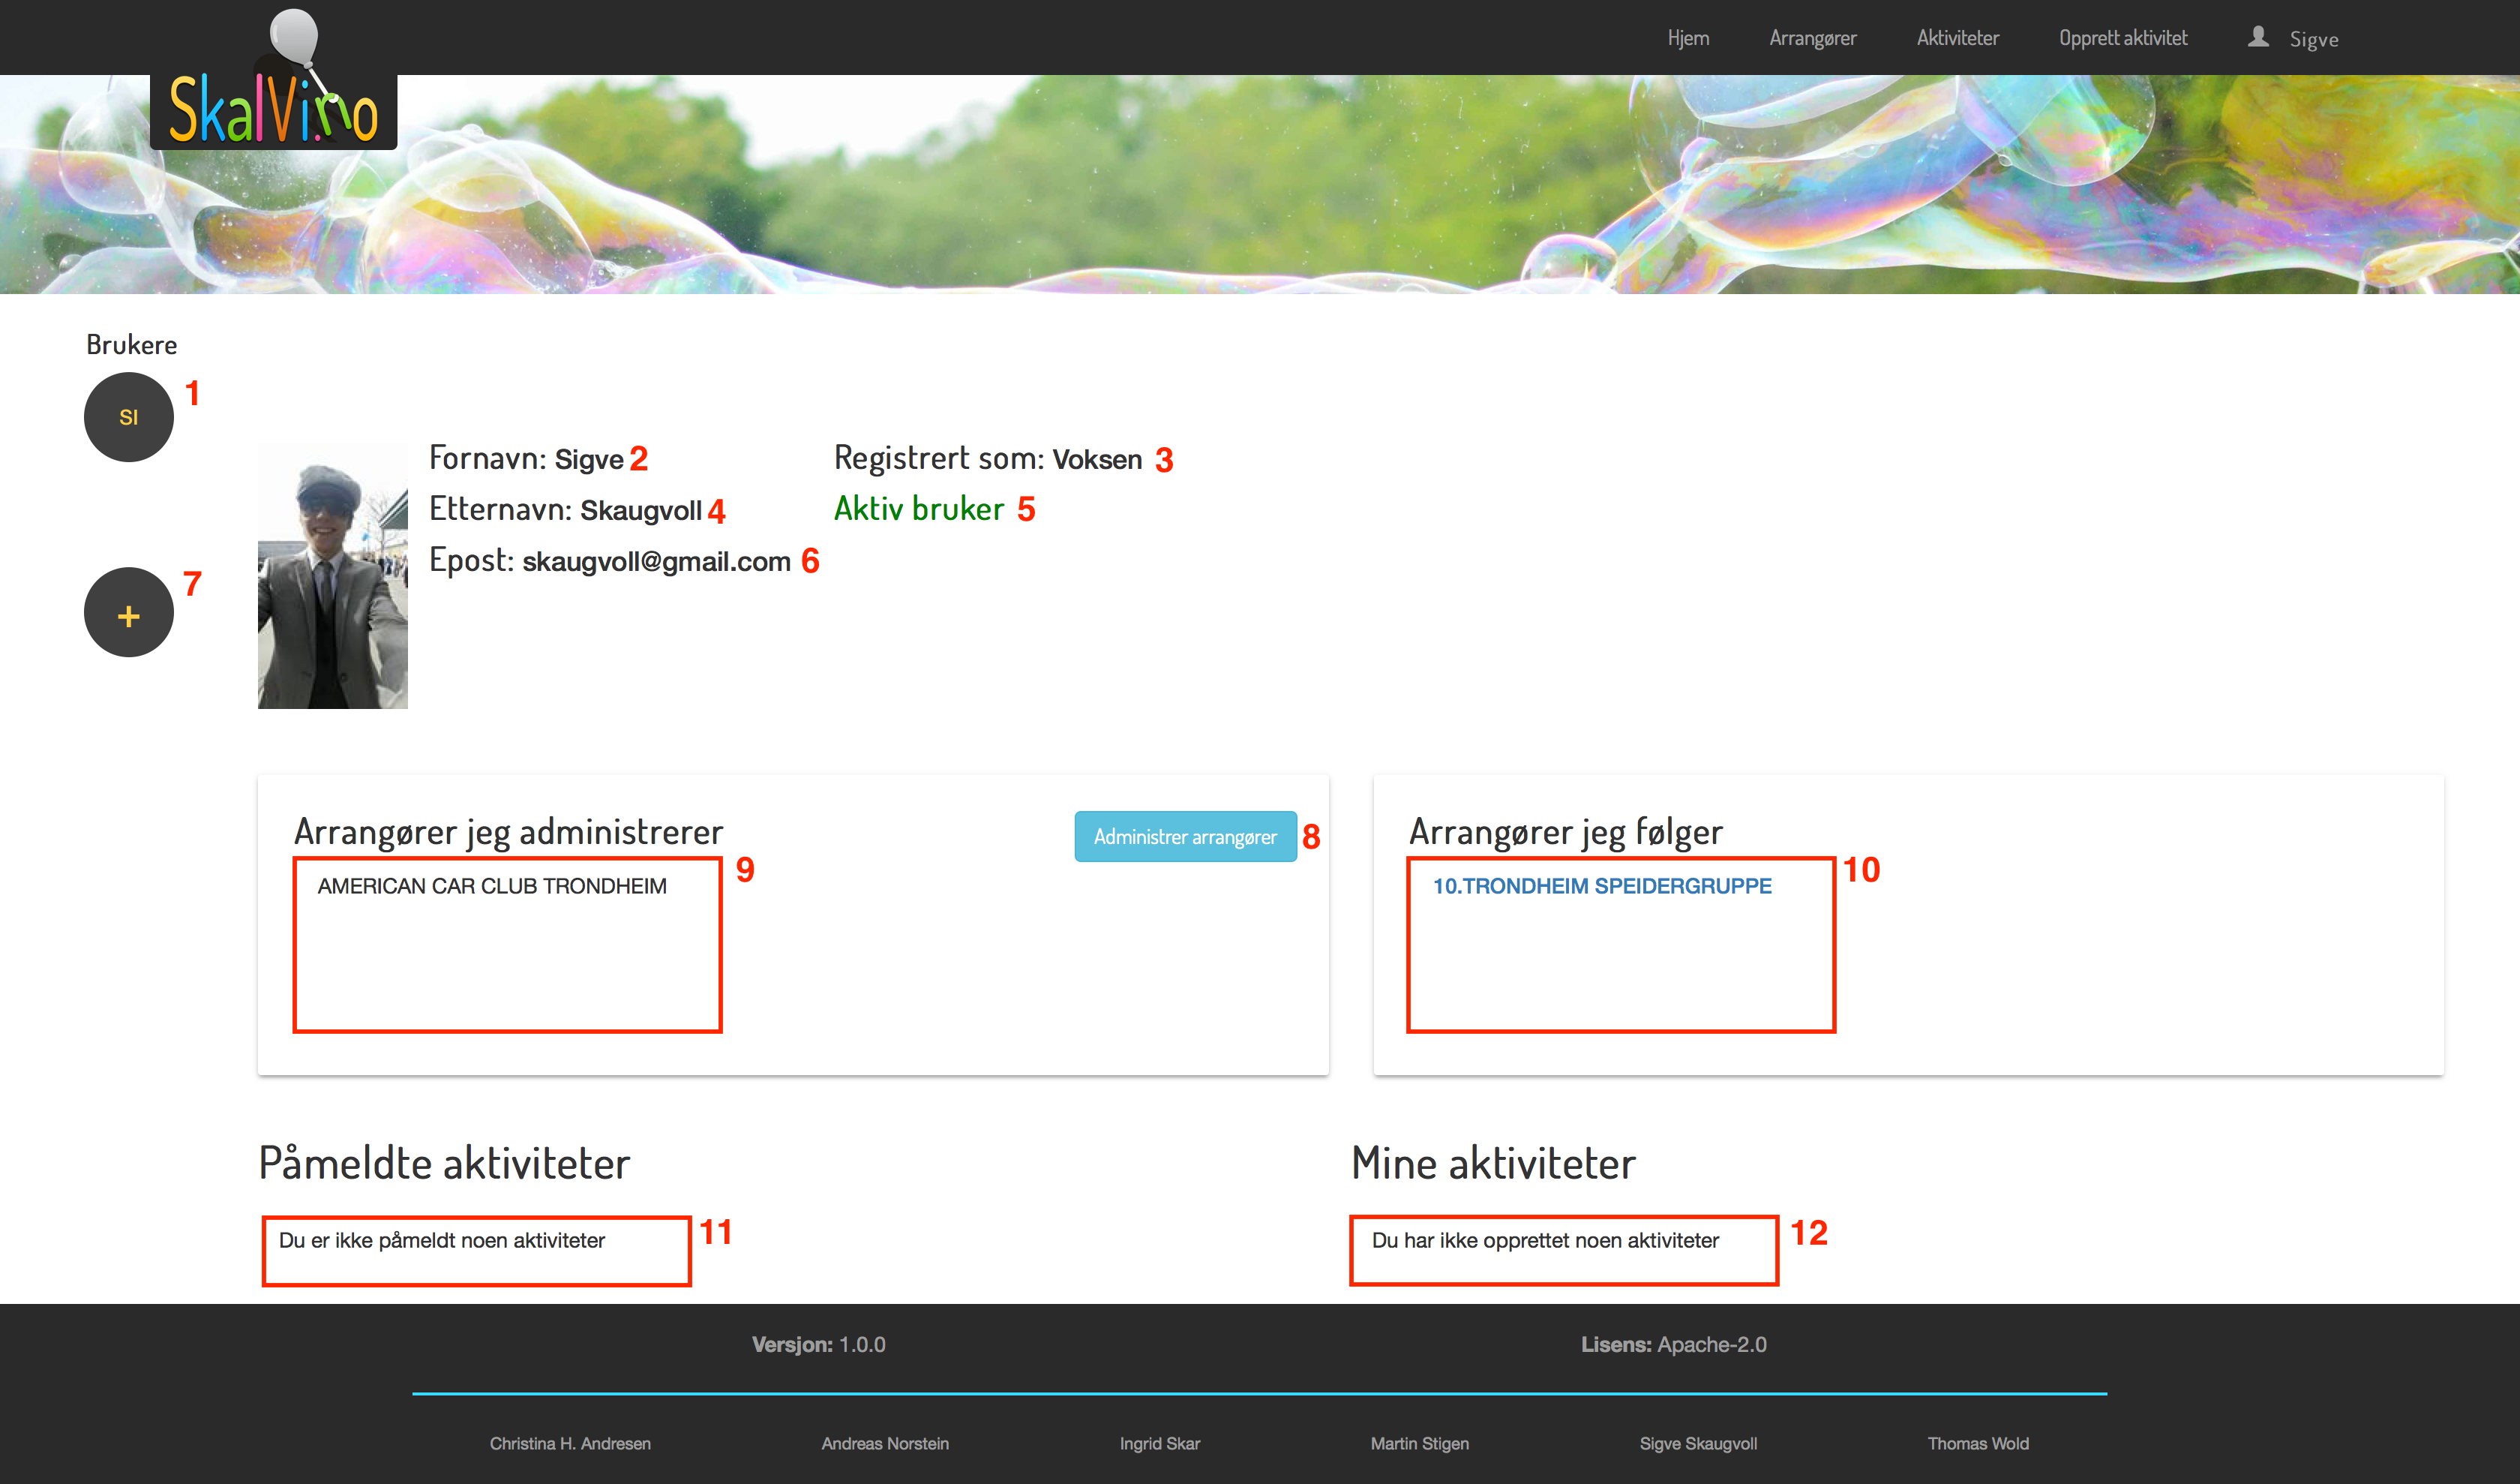
\includegraphics[height=80mm, width=\paperwidth-15mm]{appendix/manualPictures/S-myPage-Provider-cut.png}}
\end{center}
\begin{enumerate}
    \item Liste med registrerte profiler (hovedprofil og underprofiler). Bokstavene representerer første bokstaver i fornavnet til profilen.
    \item Fornavn registrert på profilen. 
    \item Hvilken type profilen er registeret som.
    \item Etternavn registrert på profilen.
    \item Viser om denne profilen er profilen som er aktiv (brukes akkurat nå).
    \item Epost som er registrert på profilen.
    \item Trykk her for å legge til en ny underprofil, som vil vises i listen (punkt 1).
    \item Trykk her for å legge til arrangører du ønsker å publisere aktiviteter på vegne av (se: administerer arrangør).
    \item Liste over registrerte arrangører profilen kan publisere aktiviteter på vegne av.
    \item Liste over arrangører profilen følger. Trykk på en arrangør for å se utfyllende informasjon om arrangøren (se: arrangør side).
    \item Liste over alle aktivitetene profilen har trykket på knappen ”Meld på” (se: modal).
    \item Liste over alle aktivitetene profilen har opprettet på Skalvi.no
\end{enumerate}

\subsection{Opprett aktivitet}
\begin{center}
  \makebox[\textwidth]{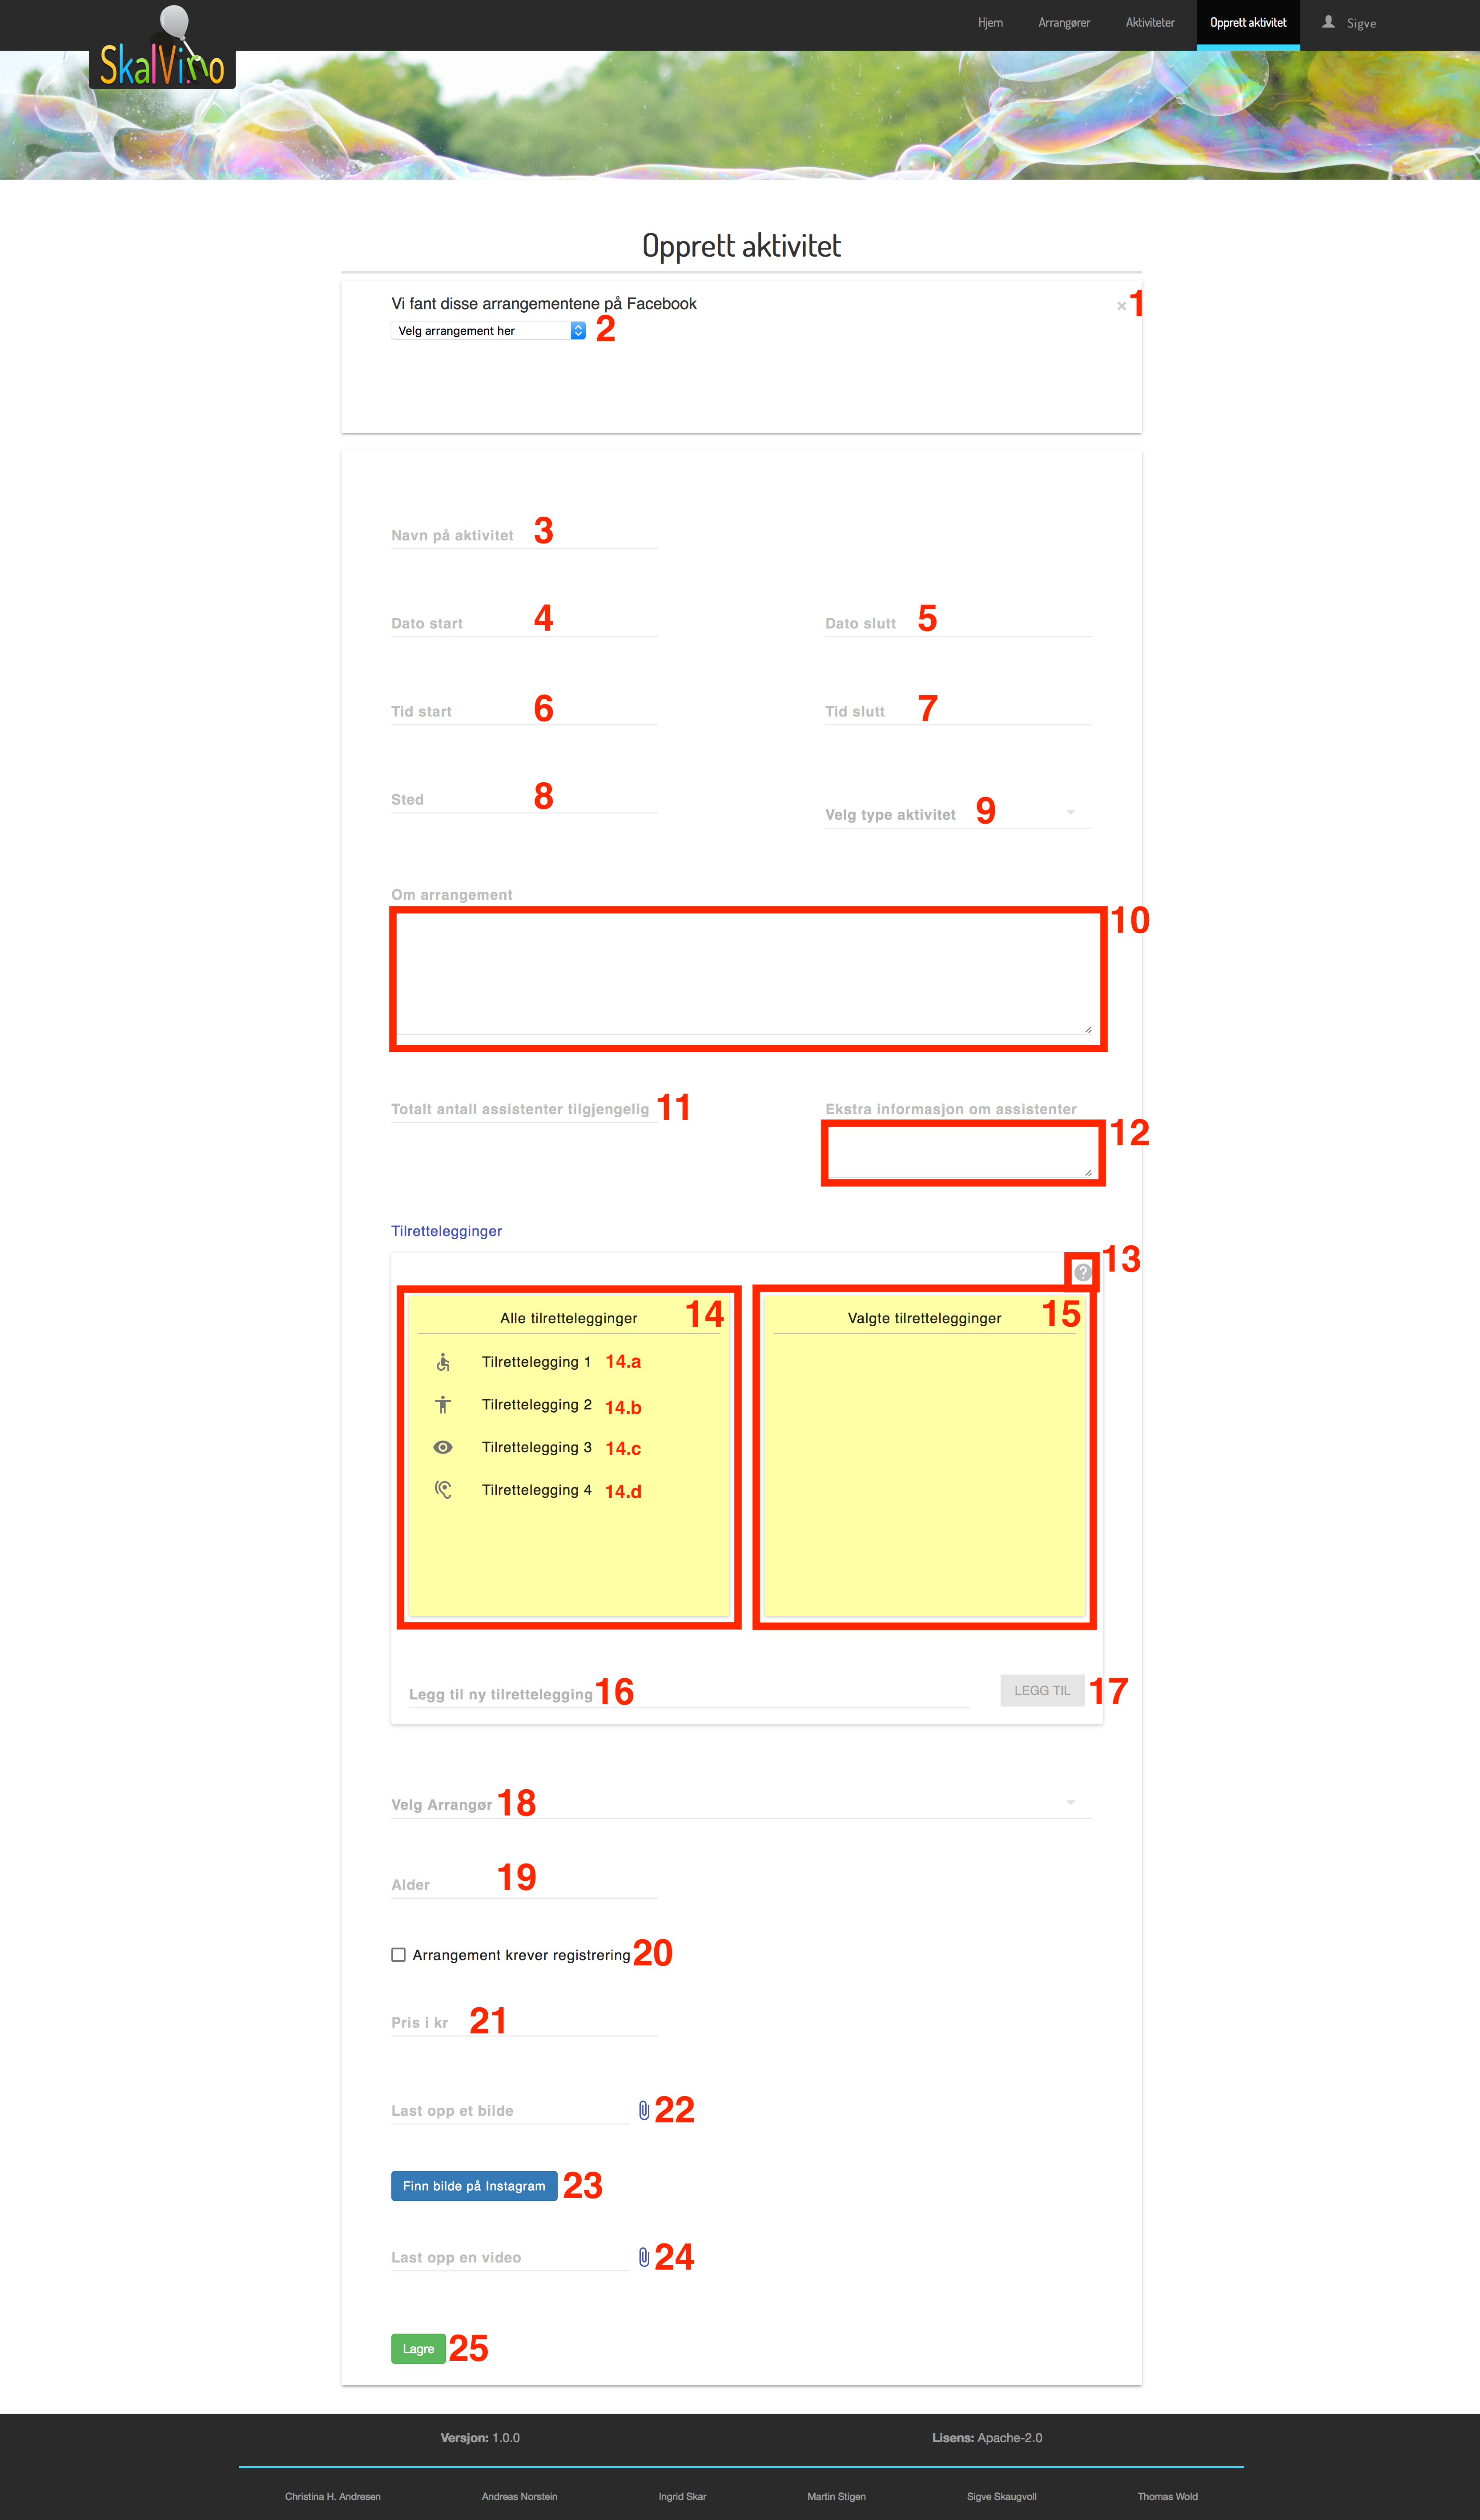
\includegraphics[height=80mm, width=\paperwidth-15mm]{appendix/manualPictures/S-newActivity-blank-cut.png}}
\end{center}
\begin{enumerate}[nosep]
    \item Trykk her får å lukke muligheten å opprette en aktivitet basert på et Facebook arrangement (kommer opp igjen, neste gang du oppretter aktivitet).
    \item Trykk her for å se liste med Facebook arrangementer du er interessert i, skal på eller har opprettet. (Hvis du velger et arrangement, må du trykke på knappen som blir synelig  rett under).
    \item Felt for å skrive inn navn på aktiviteten.
    \item Startdato for aktiviteten.
    \item Sluttdato for aktiviteten.
    \item Når på dagen aktiviteten begynner.
    \item Når på dagen aktiviteten slutter.
    \item Adressen til hvor aktiviteten skal skje.
    \item Felt for å velge hvilken type aktivitet det er. Velg blant forhånds definerte typer. Hvis ikke typen er der, velg alternativet ”annet”.
    \item Felt for å fylle inn detaljert informasjon om aktiviteten.
    \item Felt for å fylle inn hvor mange assistenter som er på aktiviteten (skal fjernes etter hvert, på grunnlag av tilbakemelding fra brukere. Se: fokusgruppe familie).
    \item Felt for å fylle inn informasjon om assistentene. (skal fjernes etter hvert, på grunnlag av tilbakemelding fra brukere. Se: fokusgruppe familie).
    \item Trykk for å få hjelp med å velge tilrettelegging for aktiviteten.
    \item Liste med forhånds definerte tilrettelegginger. (Vil etterhvert bli bare symboler, på grunnlag av tilbakemeldinger fra brukere. Se: fokusgruppe familie).
    \item Liste med valgte tilrettelegginger.
    \item Felt for å fylle inn en tilrettelegging som ikke er forhåndsdefinert (punkt 14) som skal registreres på aktiviteten.
    \item Trykk her for å registrere egendefinert tilrettelegging på aktiviteten.
    \item Felt for å velge hvem som arrangerer aktiviteten, Valg mellom profil og arrangører profilen administrerer.
    \item Felt for å angi minimum alder for aktiviteten.
    \item Trykk her for å velge at aktiviteten krever registrering / påmelding.
    \item Felt for å fylle inn hvor mye det koster å delta på aktiviteten. OBS, feltet må fylles ut, hvis aktiviteten er gratis. Skriv 0.
    \item Trykk her for å laste opp et bilde fra profilens enheten
    \item Trykk her for å laste opp et bilde fra en Instagramkonto. (NB! Funker ikke i produksjon, da det koster penger, og prosjektet enda er i ”Proof Of Concept”- fase).
    \item Trykk her for å laste opp en video fra profilens enhet.
    \item Trykk her for å registrere aktiviteten på skalvi.no.
\end{enumerate}

\subsection{Arrangør side}
\begin{center}
  \makebox[\textwidth]{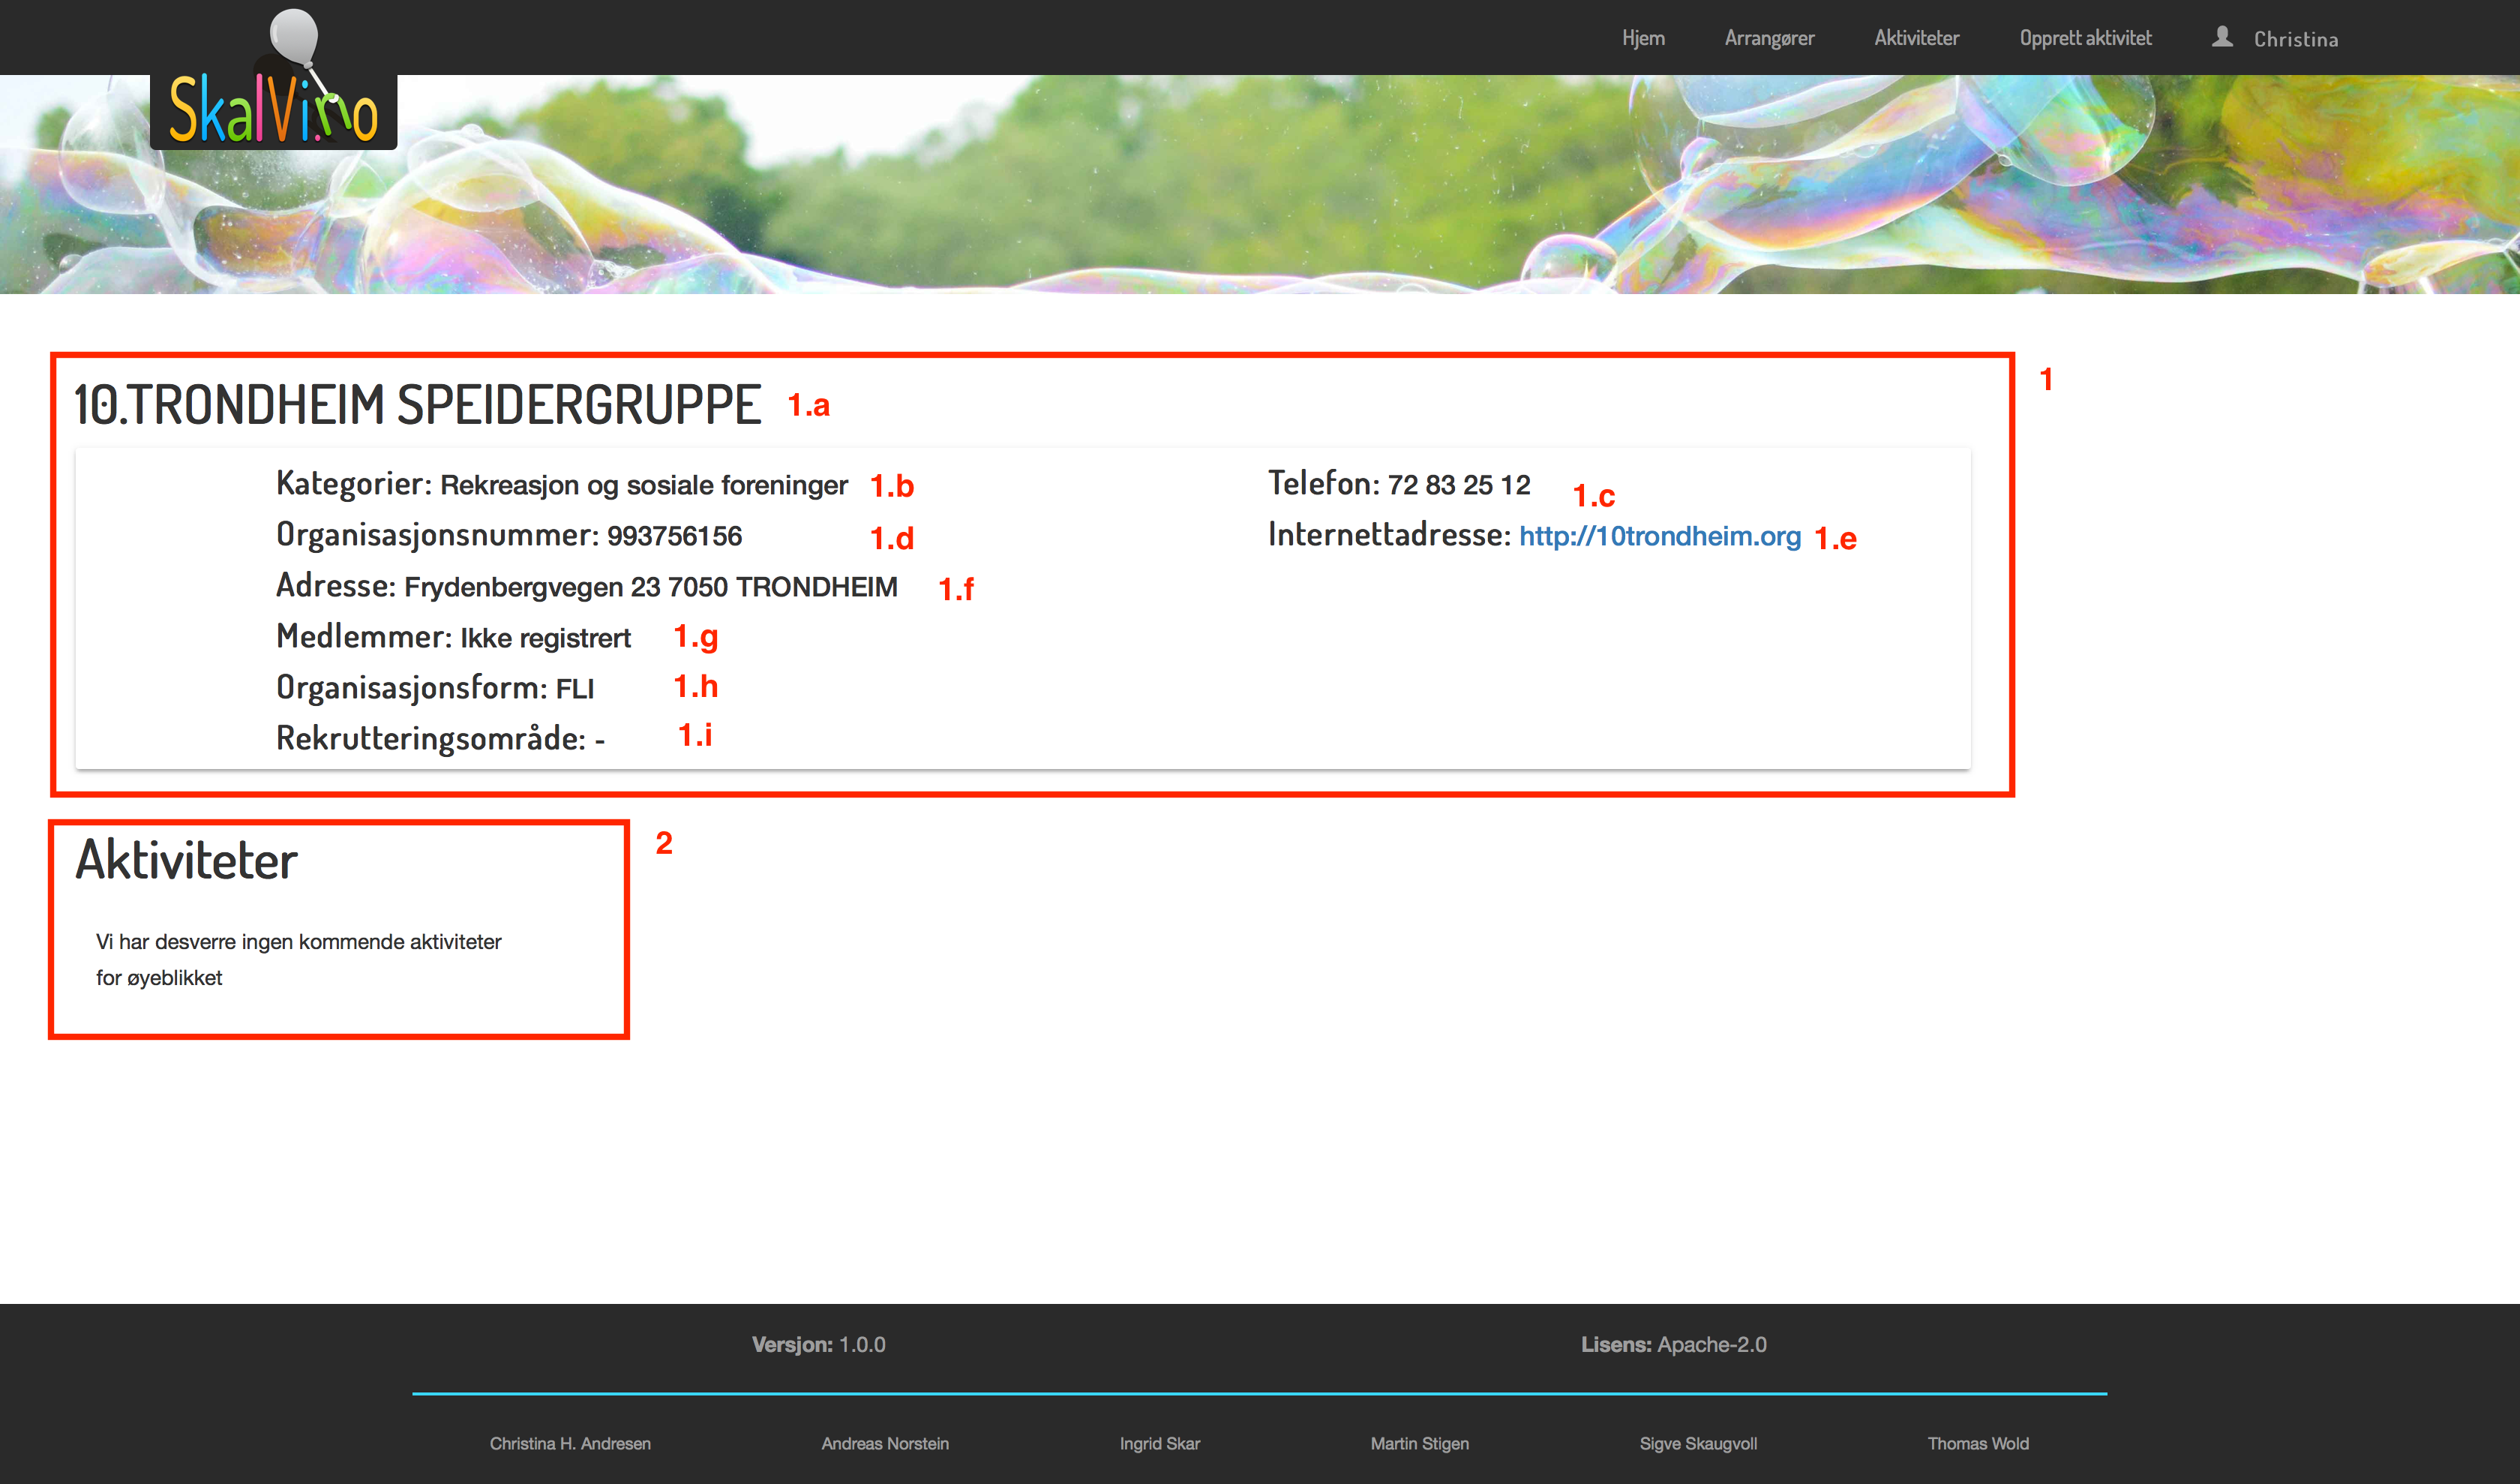
\includegraphics[height=80mm, width=\paperwidth-15mm]{appendix/manualPictures/S-Provider-page-cut.png}}
\end{center}
\begin{enumerate}
    \item Dette er en aktør, den inneholder informasjon registrert i Aktørdatabase til Trondheim Kommune. 
    \begin{enumerate}
        \item Navn på arrangør. 
        \item Hvilken kategorier arrangøren er registrert som. 
        \item Telefonnummer til arrangør.
        \item Organisasjonsnummer til arrangøren.
        \item Hjemmesiden / nettstedet til arrangøren.
        \item Hvor mange registrerte medlemmer arrangøren har. 
        \item Organisasjonsform arrangøren har.
        \item Hvor arrangøren rekrutterer.
    \end{enumerate}
    \item Her vil aktiviteter som er laget på vegne eller av arrangøren vises i en liste
\end{enumerate}




\cleardoublepage